\documentclass[english,version-2020-11]{uzl-thesis}


% Copy this file as a template for your thesis. You will have to take
% action at all places marked by
%
% !!!!!!!!!!!!!!!!!!!!!!!!!!!!!!!!!!
% !!! Your action is needed here !!!
% !!!!!!!!!!!!!!!!!!!!!!!!!!!!!!!!!!
%
% The first place your action is needed is the first line of this
% document:
%
%
% Language of the thesis:
%
% You must use either 'german' or 'english' above, depending on the
% language used in the main text. This will automatically setup a lot
% of things in the background.
%
%
% Version of the class:
%
% You must specify which version of the thesis class is to be
% used. This is important in case the class style changes in later
% years, but we still want an older thesis to look the same, even when
% things are changed in the class.
%
% Do not change or remove the version-xxxx key.
%
%
% Text encoding:
%
% Your thesis *must* be encoded in utf8 (unicode), which is the
% default in most editors these days. Do *not* change this to latin8.



%%%
%
% Main setup:
%
%%%
%
% You must use the \UzLThesisSetup command to specify numerous things
% about your thesis. This includes the entries on the title page, the 
% abstracts, and the bibliography style. You do so by specifying
% so-called "values" for so-called "keys". For instance, 
% for the key "Autor" you must provide your name as the value. You do
% so by writing 'Autor = {Max Mustermann}', that is, the value is put
% into curly braces. You can use the \UzLThesisSetup command
% repeatedly and the order in which you provide the keys is not
% important. 
%
% Everything shown on the title page must be in German -- even
% if the thesis is written in English! Just insert German text for
% German keys and English text for English keys (like 'Abstract' needs
% English text, while 'Zusammenfassung' needs German text).

\UzLThesisSetup{
  %
  % !!!!!!!!!!!!!!!!!!!!!!!!!!!!!!!!!!
  % !!! Your action is needed here !!!
  % !!!!!!!!!!!!!!!!!!!!!!!!!!!!!!!!!!
  %
  % First, specify the institut or clinic at which the thesis was
  % written. You get the logo file from them (make sure it has the
  % correct size, namely the same as the example). If they do not have
  % a logo, the university's default logo is used.
  %
  % The 'verfasst' gets two arguments. Change the first to {an der}
  % for clinics, as in 'Verfasst = {an der}{Medizinischen Klinik I}'
  %
  Logo-Dateiname        = {uzl-thesis-logo-itcs.pdf},
  Verfasst              = {am}{Institut für Software Engineering und Programming Languages},
  %
  % The titles:
  %
  Titel auf Deutsch     = {
    Können semantische Ähnlichkeiten von Wörtern die Schlussfolgerungen des gesunden Menschenverstands verbessern?  Eine Fallstudie mit Prover E und SUMO.
  }, 
  Titel auf Englisch    = {
    Can semantic similarities of words enhance common sense reasoning?  A case study with prover E and SUMO.
  },
  %
  % Author and supervisor:
  % 
  % Note that the 'Betreuer' or 'Betreuerin' is the supervisor, that
  % is, the professor who officially supervises the thesis. If there
  % is also an assistent of the professor who helped (typically a
  % lot), use 'Mit Unterstützung von' to thank that person. If the
  % thesis was mainly written 'externally' at some company or another
  % institute, point this out using 'Weitere Unterstützung'. 
  % 
  % For your own name, do *not* add things like "BSc" or "BSc
  % cand.". For the supervisor, you should normally include
  % "Prof. Dr." or "PD Dr." (ask your supervisor, what is
  % appropriate), but nothing more (so no
  % "Univ.-Prof. Dr. Dr. h.c. mult." unless your supervisor insists).  
  %
  Autor                 = {Julian Britz},
  Betreuerin            = {Prof. Dr. Diedrich Wolter},
  % 
  % Optional: Supporting persons and institutions. The text should be
  % in German, even for an English thesis.
  %
  Mit Unterstützung von = {Moritz Bayerkuhnlein},
  % 
  %   Weitere Unterstützung = {
  %     Die Arbeit ist im Rahmen einer Tätigkeit bei der Firma Muster GmbH
  %     entstanden.
  %   },
  %
  %
  % Your Degree Programm (Studiengang)
  %
  % Specify 'Bachelorarbeit' or 'Masterarbeit' and the degree
  % programme. Make sure the name of programme is correct and not
  % some abbreviation or some incorrect variant. For instance:
  % 'Medizinische Ingenierwissenschaft', but not 'MIW';
  % 'Medizinische Informatik', but not 'Medizin-Informatik';
  % 'Informatik', but not 'Informatik (SSE)'.
  %
  % Use German names for German programmes and English names for
  % English ones, so 'Infection Biology', not 'Infektionsbiologie'. 
  % For programmes that have a German bachelor and an English master,
  % use the German name for a bachelor thesis and the English name for
  % the master thesis.
  %
  Bachelorarbeit,
  Studiengang           = {Informatik},
  %
  % Date on which the thesis is turned in German, formatted the
  % traditional German way:
  %
  Datum                 = {06. Juli 2025},
  %
  % The English abstract. You must always provide abstracts in German
  % and in English. 
  %
  Abstract              = {
    Abstract
  },
  Zusammenfassung       = {
    Zusammenfassung 
  },
  %
  % Optional: 'Danksagungen' (German) or 'Acknowledgements'
  % (English). Both keys are optional and both have the same effect of
  % adding an acknowledgements text after the abstracts and before the
  % table of contents.
  %
  Acknowledgements      = {
    Ackbowledgements
  },
  % Bibliography style: Choose between
  % 
  % 'Alphabetische Bibliographie'
  % for all degree programmes in the natural sciences 
  % 
  % 'Numerische Bibliographie'
  % alternative for all other degree programmes
  % 
  % Either will load biblatex and setup the citation methods and the
  % bibliography styles correctly. You should not mess with them.
  % 
  Alphabetische Bibliographie,
  % Alternatively:
  % Numerische Bibliographie
}




%%%%%%%%%%%%%%%%%%%%
%
% Styling the thesis
%
%%%%%%%%%%%%%%%%%%%%
%
% Creating a visually pleasing layout and choosing fonts is not
% easy. Furthermore, different people have different preferences. Of
% course, for the University of Lübeck, the dean of studies could just
% force everyone to use one specific layout and font, but that seems a
% bit drastic and, also, it seems nice that thesis by different people
% have an individual style even though they all stick to the same
% overall structure.
%
% For these reasons, I (Till Tantau) have spend quite some time on
% designing a flexible layout and styling mechanism for theses.
%
% Basically, the overall structure of the thesis is fixed by the
% thesis class and so are many structural elements. For instance, you
% cannot change the order in which the abstract and table of contents
% are shown, you cannot move the bibliography elsewhere, indeed, the
% bibliography style is also fixed. Likewise, the text on the title
% page is fixed.
%
% Although many things are fixed, you *can* change several other
% things. For instance, you can change the font used for the main
% text, you can change which font is used for titles and headings or
% you can change whether titles and headlines are centered or flushed
% left.
%
% There are many LaTeX packages for changing such things. You are
% kindly asked *not to use them*. Rather, use (only) the options
% offered by the thesis class. All possible choices and combinations
% there have been tested by me and produce nice results; what happens
% with other packages no one knows and might no longer conform to what
% is expected by the university. As you will see, you still have a
% lot of options.
%
%
% Technical note: All styling is done via the command
%
% \UzLStyle{...}
%
% where ... is a key-value list just as for \UzLThesisSetup. The
% difference is just that everything having to do with styling as
% controlled by \UzLStyle, while the more “formal” setup keys are
% controlled by \UzLThesisSetup.
%
%%%
%
% Designs
%
%
% A \emph{design} is a whole set of font and layout options bundled
% together. They have been chosen in such a way that a visually
% pleasing “overall appearance” results.
%
%
% \UzLStyle{computer modern oldschool design}
%
% The look of this design mimics the “classical” way a paper or report
% created with \LaTeX\ looks like: The Computer Modern font is used,
% bold face fonts are used for headlines, only black and white are
% used as colors. This design reminds me of older scientific
% documents, especially from the computer science community where
% \LaTeX\ was used very early.
%
%
% \UzLStyle{computer modern basic design}
%
% A slightly less “oldschool” version of the previous design. It is
% still a classic design in the sense that it uses the Computer Modern
% font and that it still has this “good old \LaTeX” look, but some
% more modern aspects (like colors!) have been added.
%
% Note that this design uses Myriad for the title page (one of the
% “modern aspect”), which means that his font must be installed.
%
%
% \UzLStyle{computer modern scholary design}
%
% In my opinion, this is the ultimate “scholary design”: The thesis
% will look like it has been typeset by hand some 150 years ago and
% then printed by a university press. There is really nothing “modern”
% about it and the word in the name of the design is just part of the
% name of the “Computer Modern” font.
%
%
% \UzLStyle{pagella basic design}
%
% A, well, basic design that uses the Pagella font rather than the
% Computer Modern font. Especially the bold face version of this font
% looks nicer than the Computer Modern counterpart. Also, Pagella,
% while still having a “bookish” look, still feels a bit fresher than
% Computer Modern. 
%
%
% \UzLStyle{pagella centered design}
%
% A variant of the basic Pagella design that centers all
% headlines. A nice alternative to the basic version.
%
%
% \UzLStyle{pagella contrast design}
%
% This design tries to create some visual friction by contrasting the
% sans serif headline font (in bold!) with the main text. I find it a
% visually very interesting combination.
%
%
% \UzLStyle{alegrya basic design}
%
% The third variant of the basic design, this time using the Alegrya
% font. 
%
%
% \UzLStyle{alegrya scholary design}
%
% The Alegrya version of the previous “scholary” design. Unlike the
% Computer Modern version, this design does not look old, but more
% fresh -- while still creating the impression that the text must be
% about a very scientific subject. 
%
%
% \UzLStyle{alegrya stylish design}
%
% The design is quite similar to the scholary version for the Alegrya
% font, but with even more modern additions. “Stylish” is the word
% that comes to my mind.
%
%
\UzLStyle{alegrya modern design}
%
% A design that uses the sans serif version of the Alegrya font for
% the headlines. This is a nice modern overall design.
%
%%%




%%%%%%%%
%
% Now, include the package you need here using \usepackage. 
%
% However, many standard packages are already loaded by the class:
%
% amsmath, amssymb, amsthm, babel, biblatex, csquotes, etoolbox,
% filecontents, fontspec, geometry, hyperref, tikz (with libraries
% arrows.meta, positioning and shapes), varioref, url 
%
% Indeed, in many cases you will not need any extra packages.
%
%%%%%%%





\begin{document}

%
% The title page and table of contents will be inserted automatically
% here. 
%


\section{Introduction}

In this thesis, we investigate how adding frequently used axioms ("core axioms") to a subset of the Adimen SUMO grammar, selected based on a combination of syntactic and semantic criteria, enhances the success rate of automated theorem proving.

\subsection{Problem Statement}
\begin{itemize}
    \item Given a formal logical grammar, such as Adimen SUMO, and a conjecture $C$, we aim to determine a subset of axioms that maximizes the probability of proving $C$.
    \item We use a combination of syntactic and semantic similarity measures to select an initial set of relevant axioms $\mathcal{A}_{\text{rel}}$.
    \item We hypothesize that augmenting this set with frequently used axioms $\mathcal{A}_{\text{core}}$ further improves proof success.
\end{itemize}

\subsection{Entanglement Between Natural Language and Logical Grammar}
\begin{itemize}
    \item We do not assume a direct mapping $f: \mathcal{L}_{\text{NL}} \to \mathcal{L}_{\text{logic}}$ between natural language ($\mathcal{L}_{\text{NL}}$) and formal logic ($\mathcal{L}_{\text{logic}}$).
    \item Instead, we propose an \textbf{entanglement hypothesis}, where natural language and logical structures influence each other:
    \begin{equation}
        \mathcal{L}_{\text{NL}} \bowtie \mathcal{L}_{\text{logic}}
    \end{equation}
    \item Adimen SUMO, partially derived from WordNet, reflects structured knowledge from natural language.
    \item Natural language inherently follows logical structures, even if it remains ambiguous and context-dependent.
    \item Language models like SBERT capture semantic relationships, supporting the idea that formal logical expressions share deep structural similarities with natural language.
\end{itemize}

\subsection{Necessity of Adding Core Axioms}
\begin{itemize}
    \item To find a proof, semantic similarity alone is insufficient because logical reasoning relies on structural dependencies and inferential steps that may not be directly encoded in semantic embeddings.
    \item Theorem provers require axioms that establish intermediate logical connections because of the nature of theorem proving:
    \item Operation of Theorem Prover E
    To better understand the importance of intermediate axioms, consider how a theorem prover like E operates:
    \begin{enumerate}
        \item \textbf{Input and Preprocessing}:
        \begin{itemize}
            \item Parsing of input axioms and conjectures into a logical syntax.
            \item Conversion of formulas into conjunctive normal form (CNF) for uniformity.
        \end{itemize}
        \item \textbf{Indexing}:
        \begin{itemize}
            \item Clause indexing for efficient retrieval.
            \item Use of structures like discrimination trees for quick unification and resolution.
        \end{itemize}
        \item \textbf{Main Proof Search Loop}:
        \begin{itemize}
            \item Selection of clauses using strategies based on heuristics.
            \item Application of inference rules such as resolution and paramodulation.
            \item Simplification and subsumption of inferred clauses.
        \end{itemize}
        \item \textbf{Proof State Management}:
        \begin{itemize}
            \item Balancing expansion and reduction of search space.
            \item Employing search heuristics to efficiently explore the proof space.
        \end{itemize}
        \item \textbf{Proof Search Termination}:
        \begin{itemize}
            \item Success: Derivation of a contradiction clause indicating a proof.
            \item Failure: Resource exhaustion without finding a proof.
        \end{itemize}
        \item \textbf{Output Generation}:
        \begin{itemize}
            \item Generation of a proof object showing applied inference rules.
            \item Provision of a proof trace and performance statistics.
        \end{itemize}
    \end{enumerate}
    
    \begin{itemize}
        \item A proof is not simply a similarity-based retrieval task but requires chaining multiple inference steps to reach the desired conclusion.
        \item Many proofs require bridging axioms, which provide necessary intermediate logical steps between known premises and the conjecture.
        \item Without these bridging axioms, a theorem prover may fail to construct a proof, even if it has access to semantically relevant axioms.
    \end{itemize}
    \item The absence of intermediate axioms results in gaps in the inference chain, preventing the prover from reaching the conclusion.
    \item Empirical evidence from theorem proving suggests that missing such axioms often leads to failed proof attempts.
    \item Core axioms provide frequently used logical rules and bridges that help complete reasoning chains.
    \item Without these core axioms, proofs may fail due to missing key inference steps, even if semantically similar axioms are present.
\end{itemize}

\subsection{Formal Hypothesis}
\begin{itemize}
    \item Define:
    \begin{itemize}
        \item $\mathcal{A}$: The set of all axioms in Adimen SUMO.
        \item $C$: A conjecture to be proven.
        \item $d: \mathcal{A} \times C \to \mathbb{R}^+$: A similarity function measuring syntactic and semantic closeness.
        \item $\mathcal{A}_{\text{rel}}$: The subset of $k$ nearest axioms to $C$:
        \begin{equation}
            \mathcal{A}_{\text{rel}} = \{ A \in \mathcal{A} \mid A \text{ is among the } k \text{ closest axioms to } C \text{ w.r.t. } d \}
        \end{equation}
        \item $\mathcal{A}_{\text{core}}$: A set of frequently used axioms in previous proofs.
        \item $\mathcal{A}_{\text{enh}} = \mathcal{A}_{\text{rel}} \cup \mathcal{A}_{\text{core}}$: The enhanced axiom set.
        \item $P(T, \mathcal{A}', C)$: A function that returns $\text{True}$ if theorem prover $T$ finds a proof of $C$ using $\mathcal{A}'$, otherwise $\text{False}$.
    \end{itemize}
    \item Hypothesis:
    \begin{equation}
        \forall C \in \mathcal{C}, \quad \Pr(P(T, \mathcal{A}_{\text{enh}}, C) = \text{True}) > \Pr(P(T, \mathcal{A}_{\text{rel}}, C) = \text{True})
    \end{equation}
    \item This suggests that the success probability of proving $C$ increases when $\mathcal{A}_{\text{core}}$ is included.
\end{itemize}

\subsection{Justification and Implications}
\begin{itemize}
    \item Since Adimen SUMO’s grammar is \textbf{entangled} with natural language structures, selecting axioms using semantic embeddings (e.g., SBERT) captures implicit logical dependencies.
    \item Frequently used axioms act as \textbf{structural anchors} within this entanglement, improving proof discovery.
    \item The theorem prover benefits from both the \textbf{nearest axioms} and the \textbf{core axioms}, leading to an overall higher proof success rate.
\end{itemize}

This thesis aims to empirically validate this hypothesis by evaluating proof success rates with different axiom selection strategies and demonstrating the effectiveness of incorporating core axioms.




% DELETE the following line for your own thesis - it causes trouble!
\lstMakeShortInline[style=code,style=inline,language={[LaTeX]tex},moretexcs={chapter}]|


\section{Related Work}
% In a German thesis write: \section{Verwandte Arbeiten}
  \cite{Schon2024}
  \cite{Àlvez2014}
  \cite{Hoder2011}
  \cite{Roederer2009}
  \cite{Sutcliffe2007}
% !!!!!!!!!!!!!!!!!!!!!!!!!!!!!!!!!!
% !!! Your action is needed here !!!
% !!!!!!!!!!!!!!!!!!!!!!!!!!!!!!!!!!
%
% Replace with a detailed account of what other people have already
% researched concerning your thesis's theme. Even when (indeed,
% especially when) there has been only little or even no research by
% other people, you should explain in detail that this is the case and
% why it is the case. 


\section{Structure of this Thesis}
% In a German thesis write: \section{Aufbau dieser Arbeit}


Structure of this Thesis.



% !!!!!!!!!!!!!!!!!!!!!!!!!!!!!!!!!!
% !!! Your action is needed here !!!
% !!!!!!!!!!!!!!!!!!!!!!!!!!!!!!!!!!
%
% Replace the whole text chapter with the main text of your thesis! 

\chapter{Preliminaries}
\label{chapter-use}

  \section{Common Sense Reasoning}
  \begin{itemize}
      \item \textbf{Explanation:} Common sense reasoning refers to the ability of a system to make presumptions about the everyday world, similar to human reasoning.
      \item \textbf{What is it?} It involves reasoning about typical situations, handling incomplete information, and making reasonable assumptions.
      \item \textbf{Applications and Use Cases:}
      \begin{itemize}
          \item Natural language understanding.
          \item Automated reasoning.
          \item Robotics and AI decision-making.
      \end{itemize}
      \item \textbf{Current State:} Modern AI systems, including deep learning models, struggle with common sense reasoning, but efforts such as knowledge graphs and large-scale pre-trained models aim to improve it.
      \item \textbf{Challenges:}
      \begin{itemize}
          \item Ambiguity in natural language.
          \item Lack of structured common-sense knowledge.
          \item Computational limitations in reasoning.
      \end{itemize}
  \end{itemize}

  \section{Word Embeddings}
    \begin{itemize}
        \item \textbf{Definition:} Word embeddings are dense vector representations of words that capture semantic meanings.
        \item \textbf{Creation:} Generated using neural network-based models like Word2Vec, GloVe, and FastText.
        \item \textbf{Properties:}
          \begin{itemize}
              \item Captures semantic similarity.
              \item Enables algebraic operations like \textit{king - man + woman = queen}.
          \end{itemize}
        \item \textbf{Applications:}
          \begin{itemize}
              \item Natural language processing (NLP).
              \item Machine translation.
              \item Information retrieval.
          \end{itemize}
        \item \textbf{Limitations and Challenges:}
          \begin{itemize}
              \item Contextual ambiguity.
              \item Bias in training data.
              \item Scalability for large vocabularies.
          \end{itemize}
    \end{itemize}

  \section{Grammars}
    \begin{itemize}
        \item \textbf{Explanation:} Grammars define the structure and rules governing a language, whether natural or formal.
        \item \textbf{Types of Grammars:} Context-free grammars, dependency grammars, formal grammars.
        \item \textbf{Structure and Organization:} Grammars consist of syntax rules, lexicons, and transformations.
        \item \textbf{Why Are They Needed?} They provide the foundation for parsing, generating, and interpreting language in NLP and logic systems.
        \item \textbf{SUMO:} Suggested Upper Merged Ontology, a formal ontology integrating linguistic and logical structures.
    \end{itemize}

  \section{Theorem Provers}
    \begin{itemize}
        \item \textbf{Explanation:} Theorem provers are automated reasoning tools designed to validate logical statements based on formal rules.
        \item \textbf{Types of Theorem Provers:} Resolution-based, tableau-based, and interactive provers.
        \item \textbf{Functionality:} They work by refutation—attempting to derive contradictions from the negation of a theorem.
        \item \textbf{Why Are They Needed?} Essential for verifying mathematical proofs, formal verification, and logic-based AI.
        \item \textbf{Limits and Challenges:}
        \begin{itemize}
            \item Computational complexity.
            \item Handling undecidable problems.
            \item Scalability for large proof spaces.
        \end{itemize}
        \item \textbf{Prover E:}
        \begin{itemize}
            \item \textbf{How Does E Work?} A saturation-based theorem prover using superposition calculus.
            \item \textbf{Satauto Mode:} An automatic mode that selects strategies dynamically for proof search.
        \end{itemize}
    \end{itemize}

  \section{Selection Strategies}
    \begin{itemize}
        \item \textbf{Syntactic:} Selects axioms based on structural similarity and pattern matching.
        \item \textbf{Semantic:} Uses embeddings and meaning-based similarity to find relevant axioms.
        \item \textbf{Combination - Union:} Integrates syntactic and semantic methods to enhance selection efficiency.
    \end{itemize}



\chapter{Experiments}
    %
    \section{How WhiteboxTests are made}
      \begin{itemize}
        \item Paper of Álvez about building WhiteBox Tests \cite{Álvez2017}
        \begin{enumerate}
          \item In the context of Adimen SUMO, \textbf{falsity tests} are formulated by taking specific statements or conditions and applying \textbf{negation} to them.
          \item These negated statements serve as a basis for falsity tests, which are essential in logical proof systems.
          \item A \textbf{theorem prover} such as Prover E then performs a process known as \textbf{refutation}.
          \item Through refutation, the theorem prover attempts to demonstrate the \textbf{inconsistency} or \textbf{falsehood} of the original statements.
          \item This is achieved by attempting to derive a \textbf{contradiction} from the negated statements, indicating that the original (non-negated) statements cannot all be true simultaneously.
        \end{enumerate}
      \end{itemize}
    %
    \section{Reengineering of paper \cite{Schon2024}}
      \begin{figure}[h!]
        \centering
        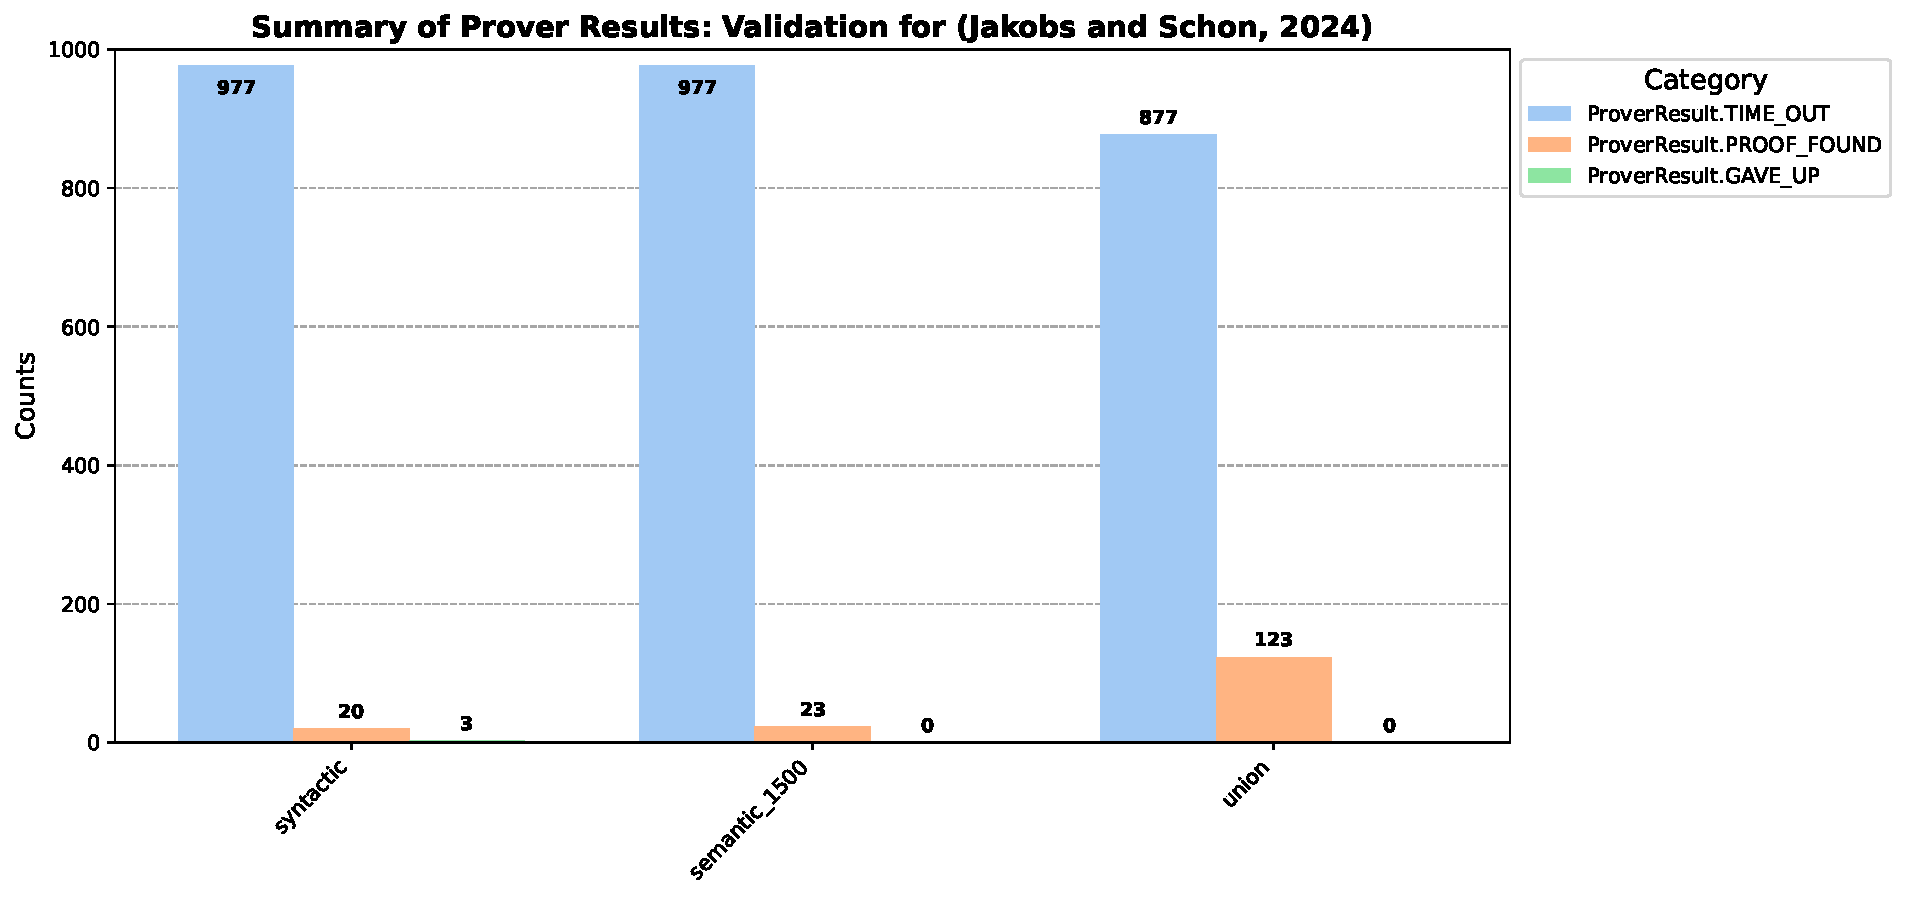
\includegraphics[width=\textwidth]{standard_mode_noAdded_output.pdf} % Add path to the PDF image
        \caption{Reengineering of results of paper \cite{Schon2024}}
        \label{fig:reengineering}
      \end{figure}
      \clearpage
    %
    \section{Analyze of reeingineering}
      \begin{itemize}
        \item Mean variable count
          \begin{figure}[h!]
            \centering
            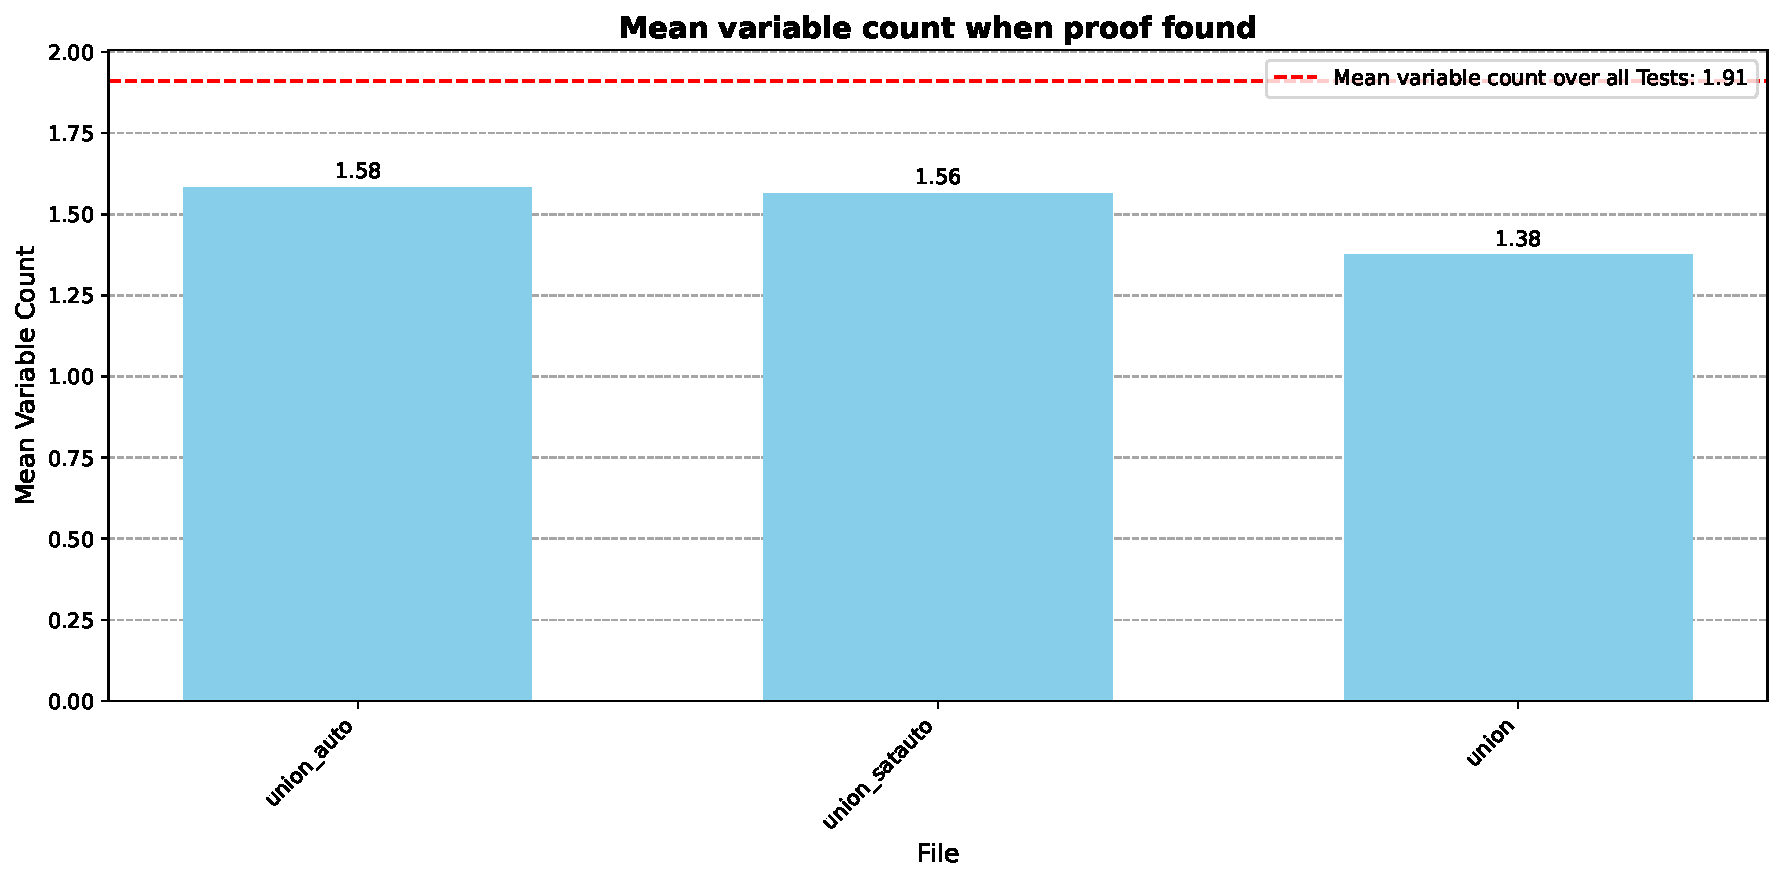
\includegraphics[width=\textwidth]{variable_count.pdf} % Add path to the PDF image
            \caption{Variable Count}
            \label{fig:variable_count}
          \end{figure}
        \item Count signs
          \begin{figure}[h!]
            \centering
            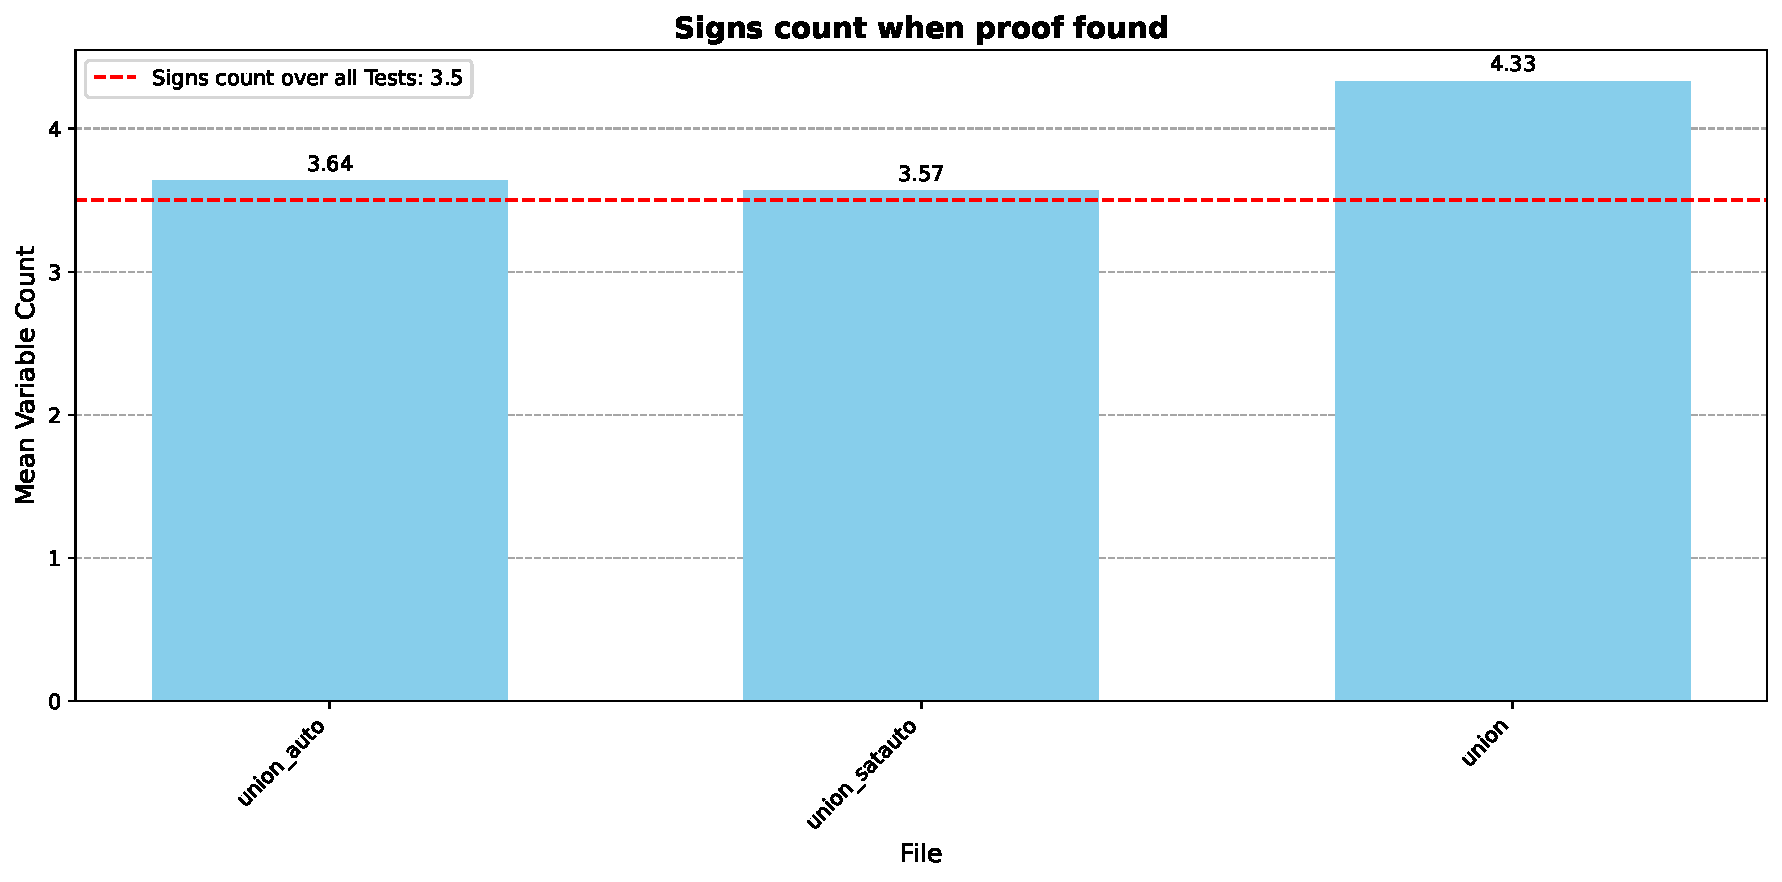
\includegraphics[width=\textwidth]{signs_count.pdf} % Add path to the PDF image
            \caption{Count signs}
            \label{fig:count_signs}
          \end{figure}
        \item Character Count
          \begin{figure}[h!]
            \centering
            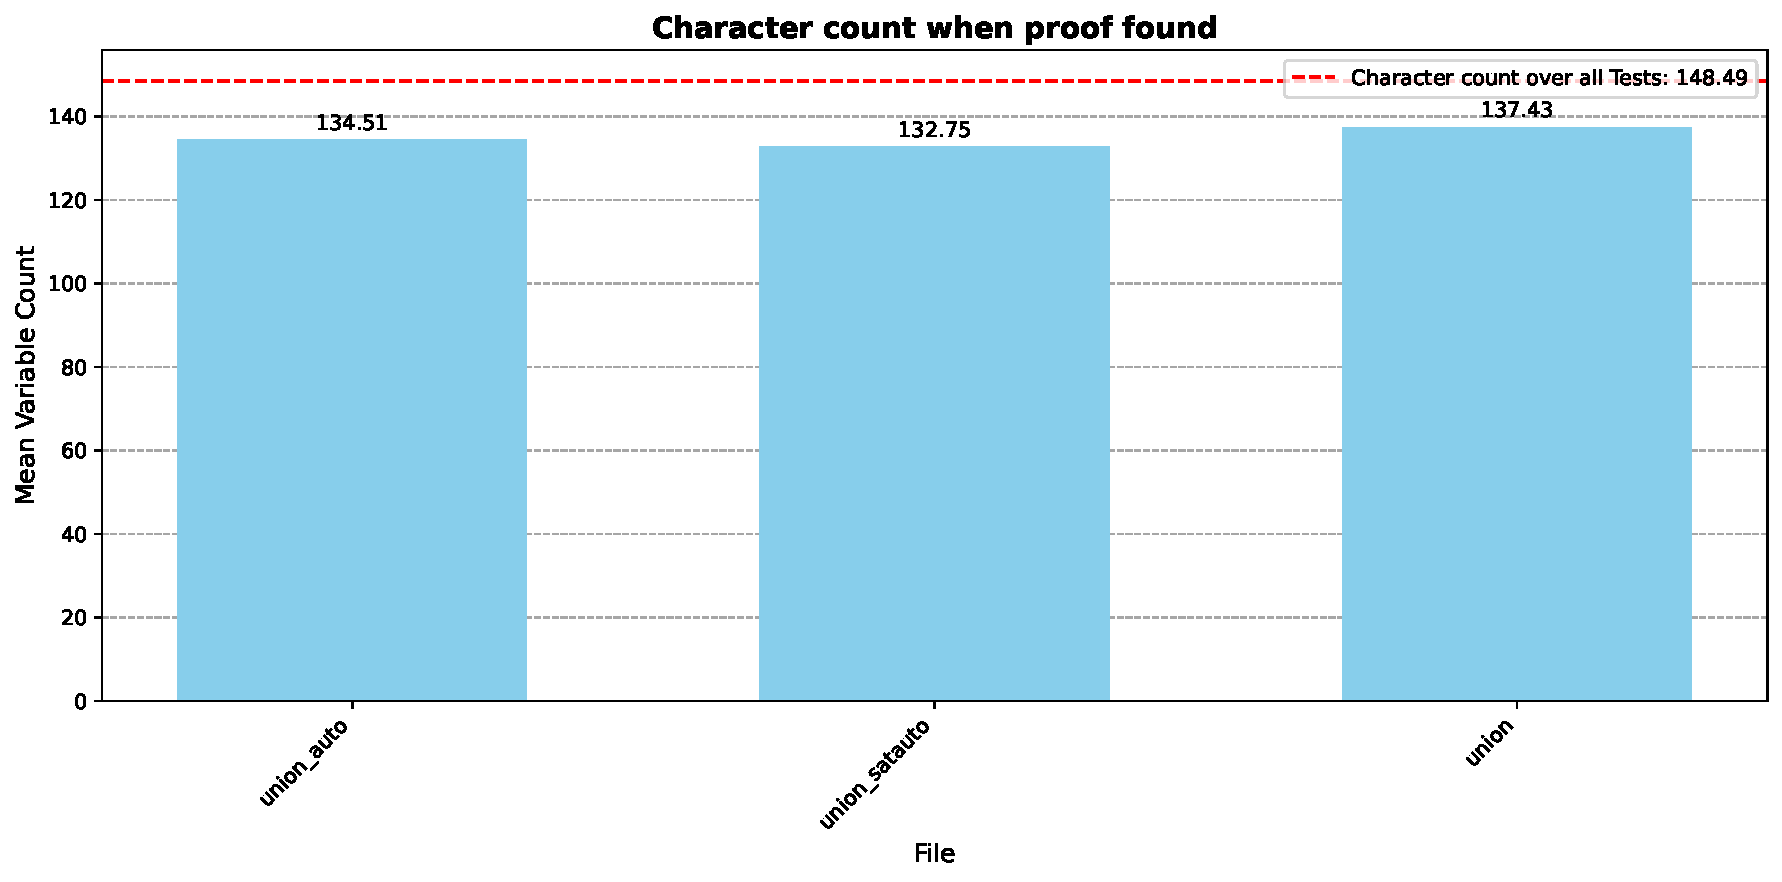
\includegraphics[width=\textwidth]{character_count.pdf} % Add path to the PDF image
            \caption{Character count}
            \label{fig:character_count}
          \end{figure}
          \clearpage
        \item Cosine similarity
          \begin{figure}[h!]
            \centering
            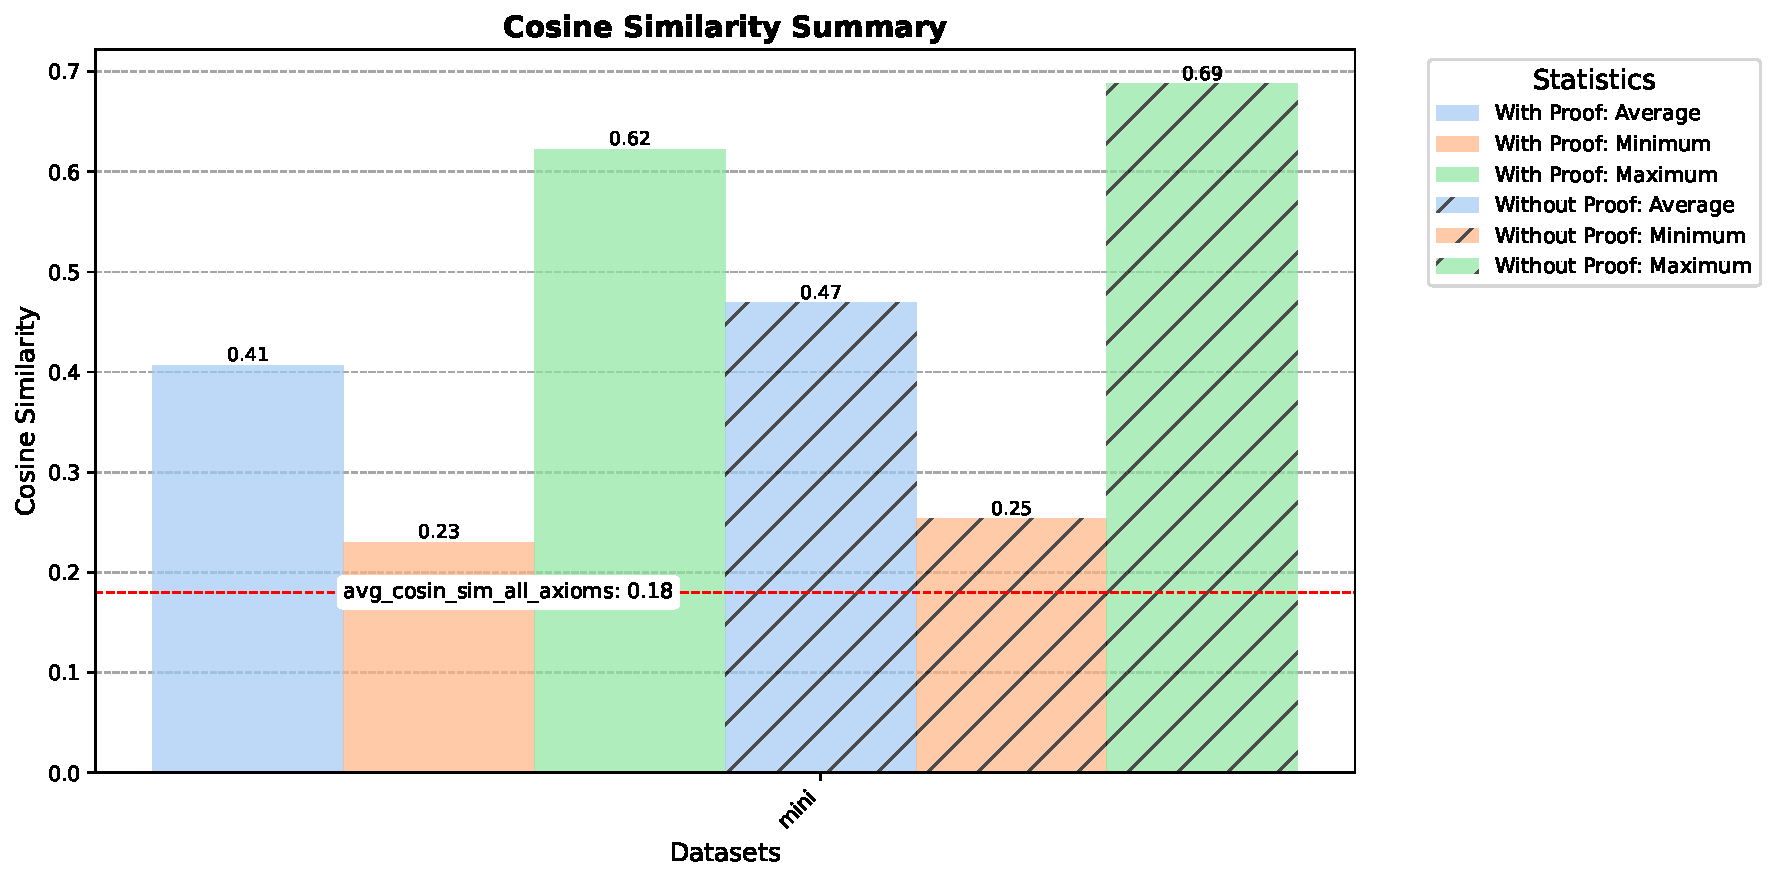
\includegraphics[width=\textwidth]{cosine_similarity_mini_noAdded_summary.pdf} % Add path to the PDF image
            \caption{Cosine similarity}
            \label{fig:cosine_similarity}
          \end{figure}
          Why Would Provable Conjectures Have Lower Axiom Similarity? This suggests that proving the conjecture involves bridging different concepts, rather than just refining a single closely related idea.
          \clearpage
      \end{itemize}
    %
    \section{Add core axioms}
      \begin{itemize}
        \item Results of prover
          \begin{figure}[h!]
            \centering
            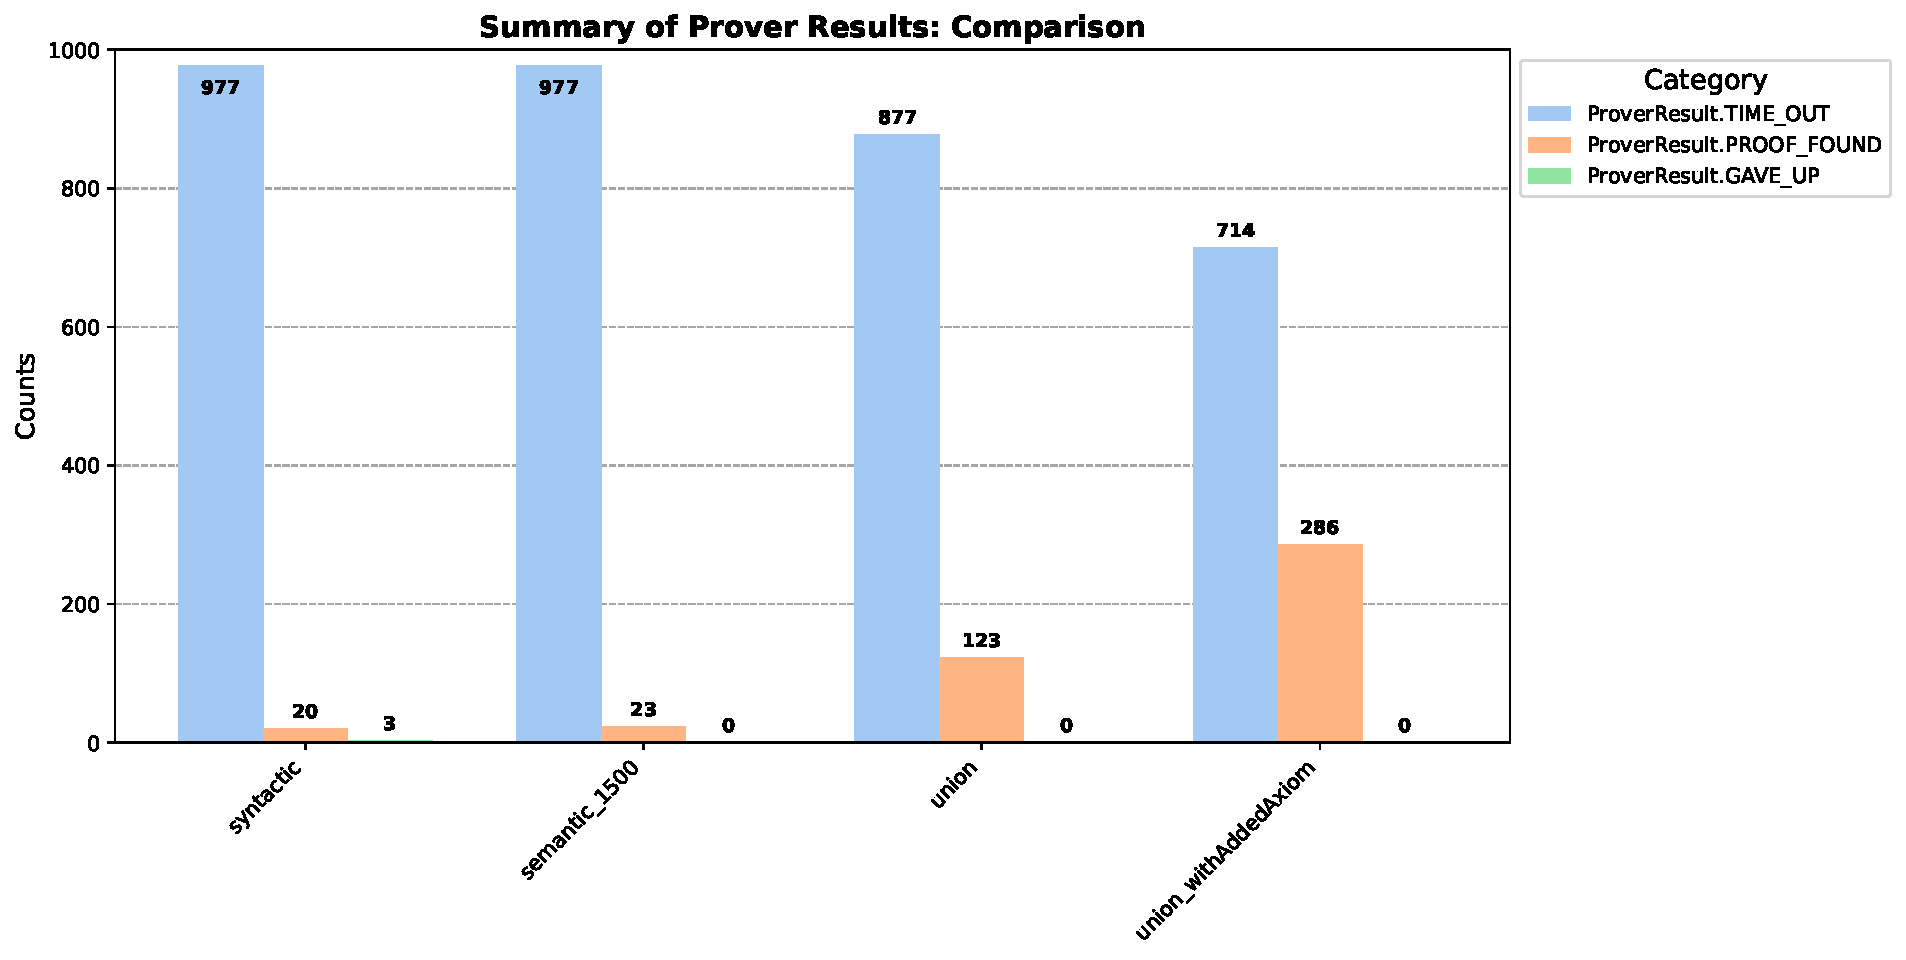
\includegraphics[width=\textwidth]{standard_mode_output.pdf} % Add path to the PDF image
            \caption{Summary of Prover Results with core axioms}
            \label{fig:prover_results_with_core_axioms}
          \end{figure}
        \item Cosine similarity
          \begin{figure}[h!]
            \centering
            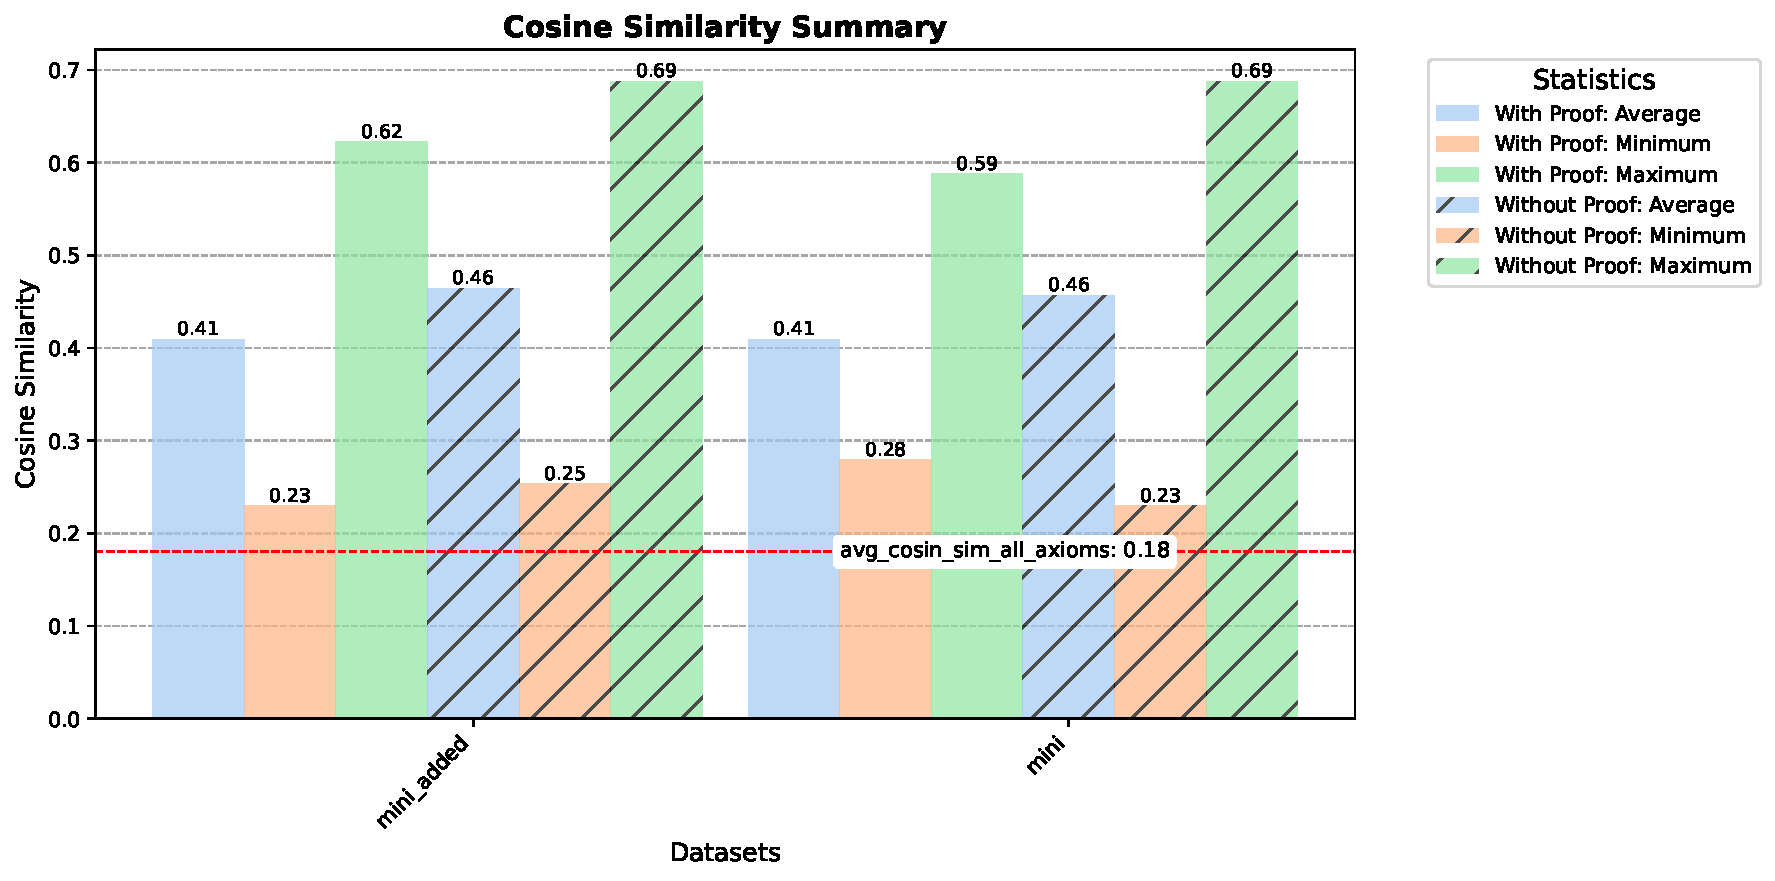
\includegraphics[width=\textwidth]{cosine_similarity_mini_summary.pdf} % Add path to the PDF image
            \caption{Summary of Prover Results: Standard Mode}
            \label{fig:prover_results_standard}
          \end{figure}
        \clearpage
      \end{itemize}
    %
    \section{Comparing LLMs}
      \begin{itemize}
        \item Results of prover
          \begin{figure}[h!]
            \centering
            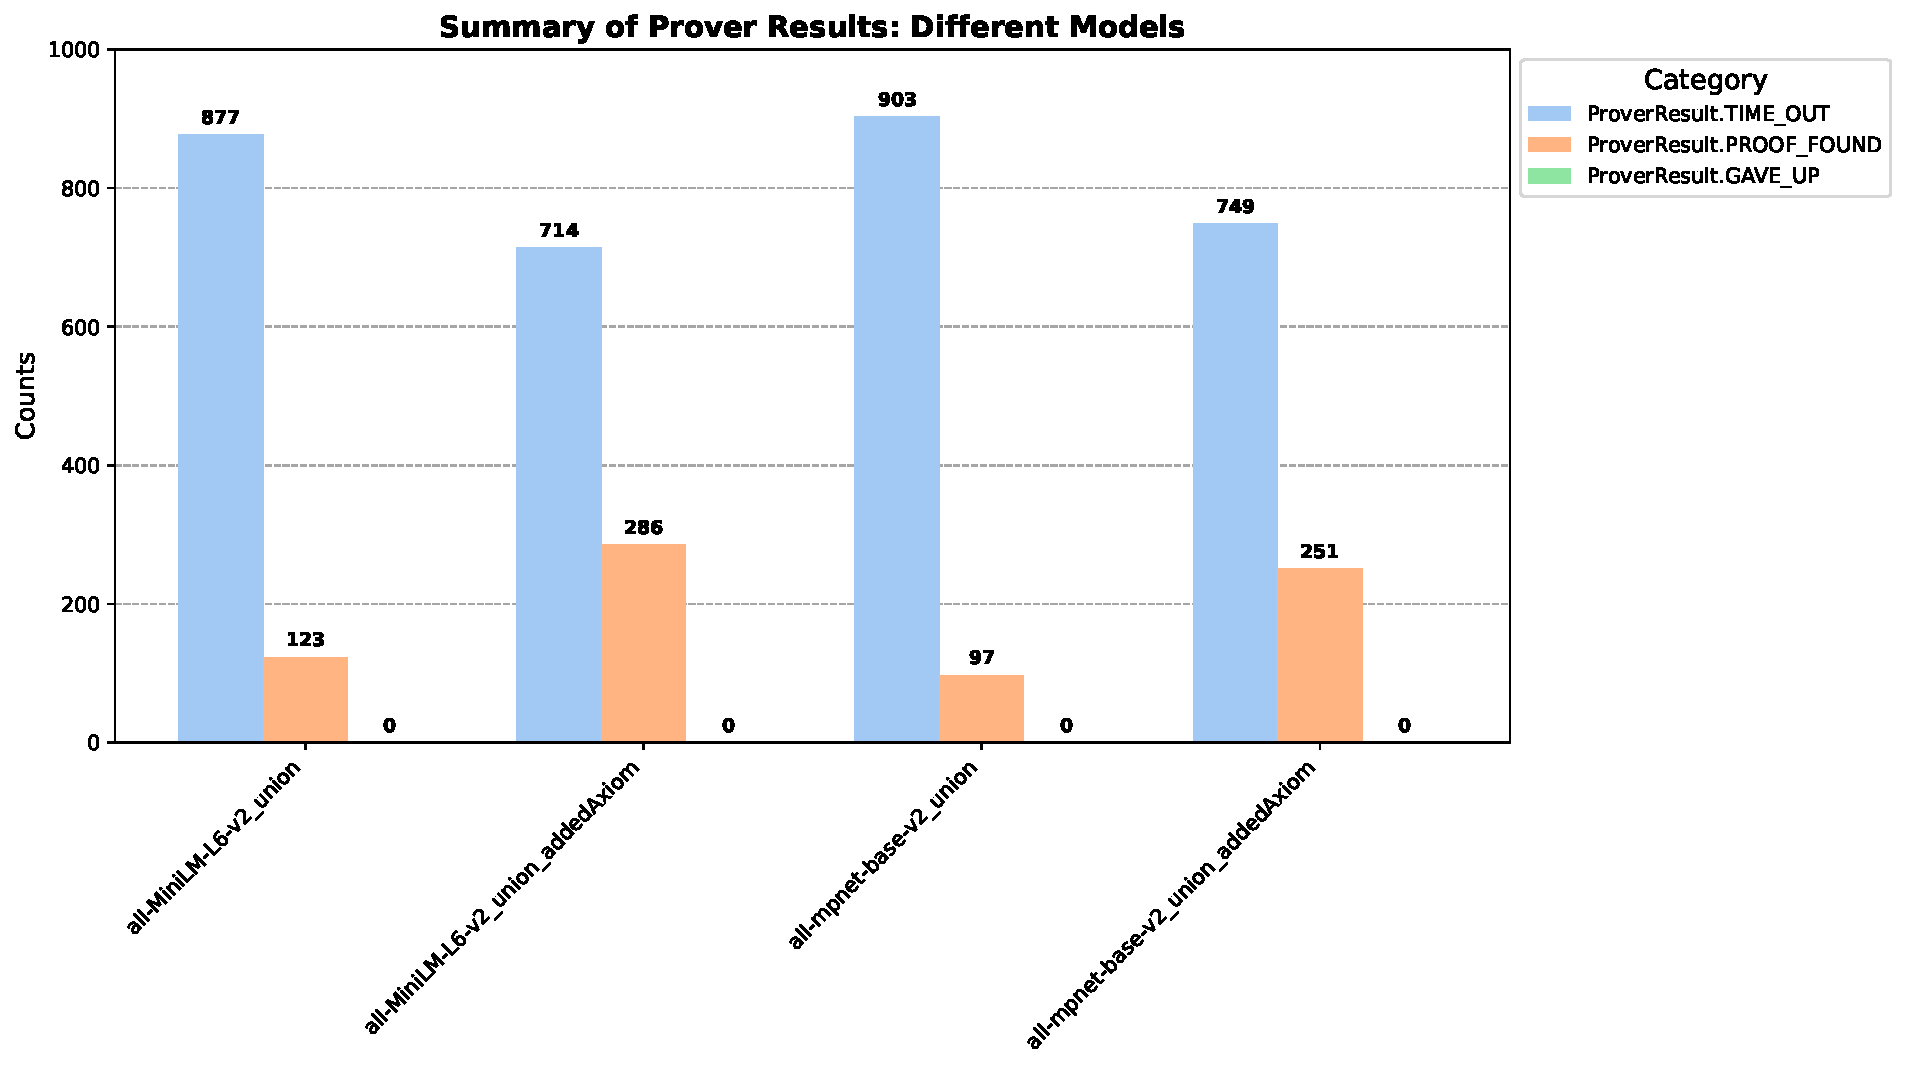
\includegraphics[width=\textwidth]{different_mode_output.pdf} % Add path to the PDF image
            \caption{Summary of Prover Results: Different models}
            \label{fig:results_different_models}
          \end{figure}
        \item Cosine similarity
          \begin{figure}[h!]
            \centering
            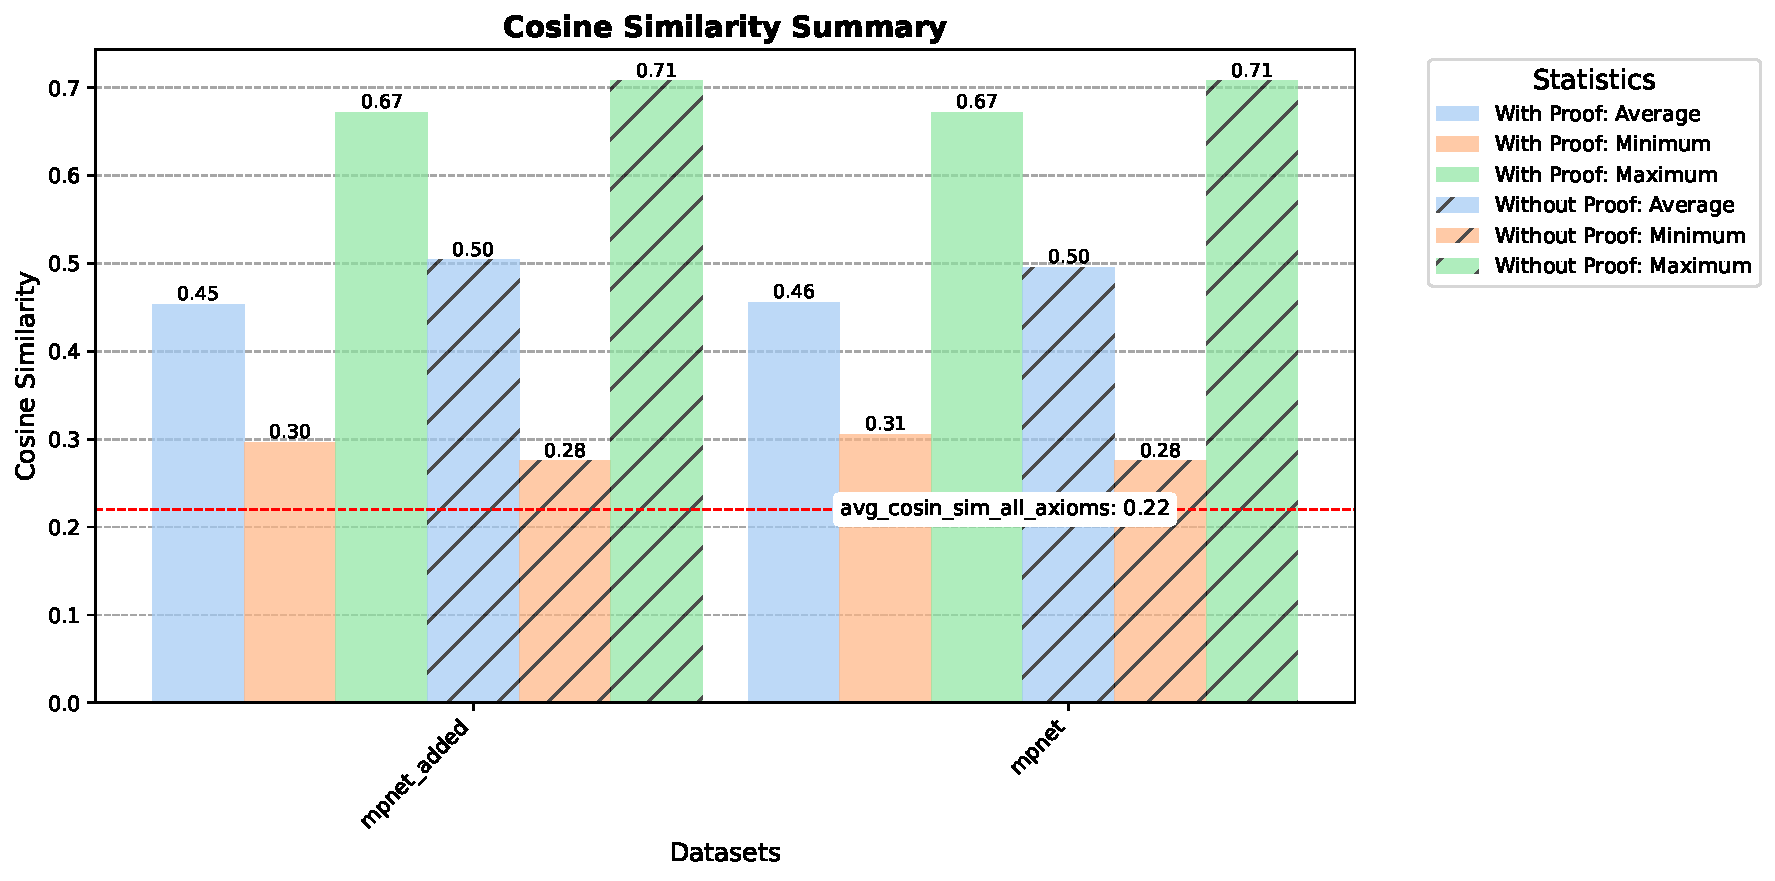
\includegraphics[width=\textwidth]{cosine_similarity_mpnet_summary.pdf} % Add path to the PDF image
            \caption{Cosine Similarity Mpnet}
            \label{fig:cosine_similarity_mpnet}
          \end{figure}
          \clearpage
      \end{itemize}
    %
    \section{Analyze different E settings}
      \begin{itemize}
        \item Satauto
          Using search heuristic
          \begin{figure}[h!]
            \centering
            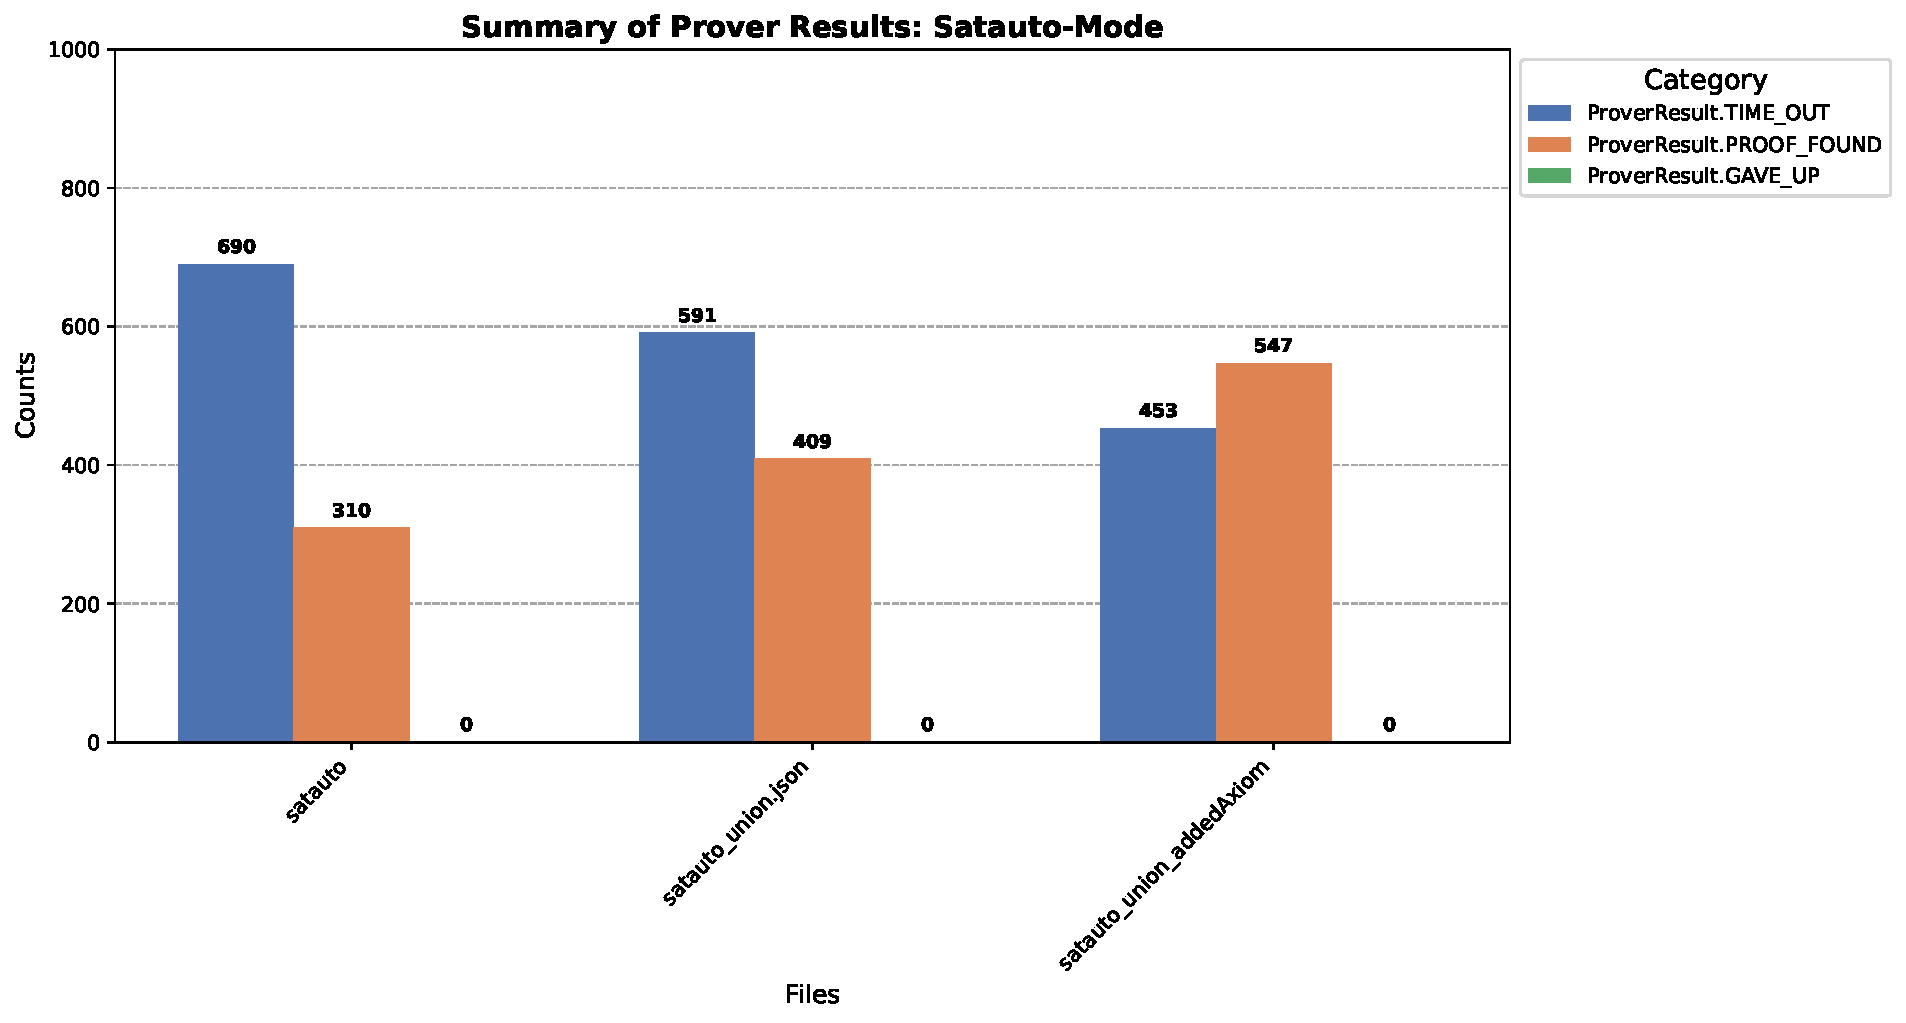
\includegraphics[width=\textwidth]{satauto_mode_output.pdf} % Add path to the PDF image
            \caption{Summary of Prover Results: Satauto Mode}
            \label{fig:prover_results_satauto}
          \end{figure}
        \item Auto
          Using SInE + search heuristic
          \begin{figure}[h!]
            \centering
            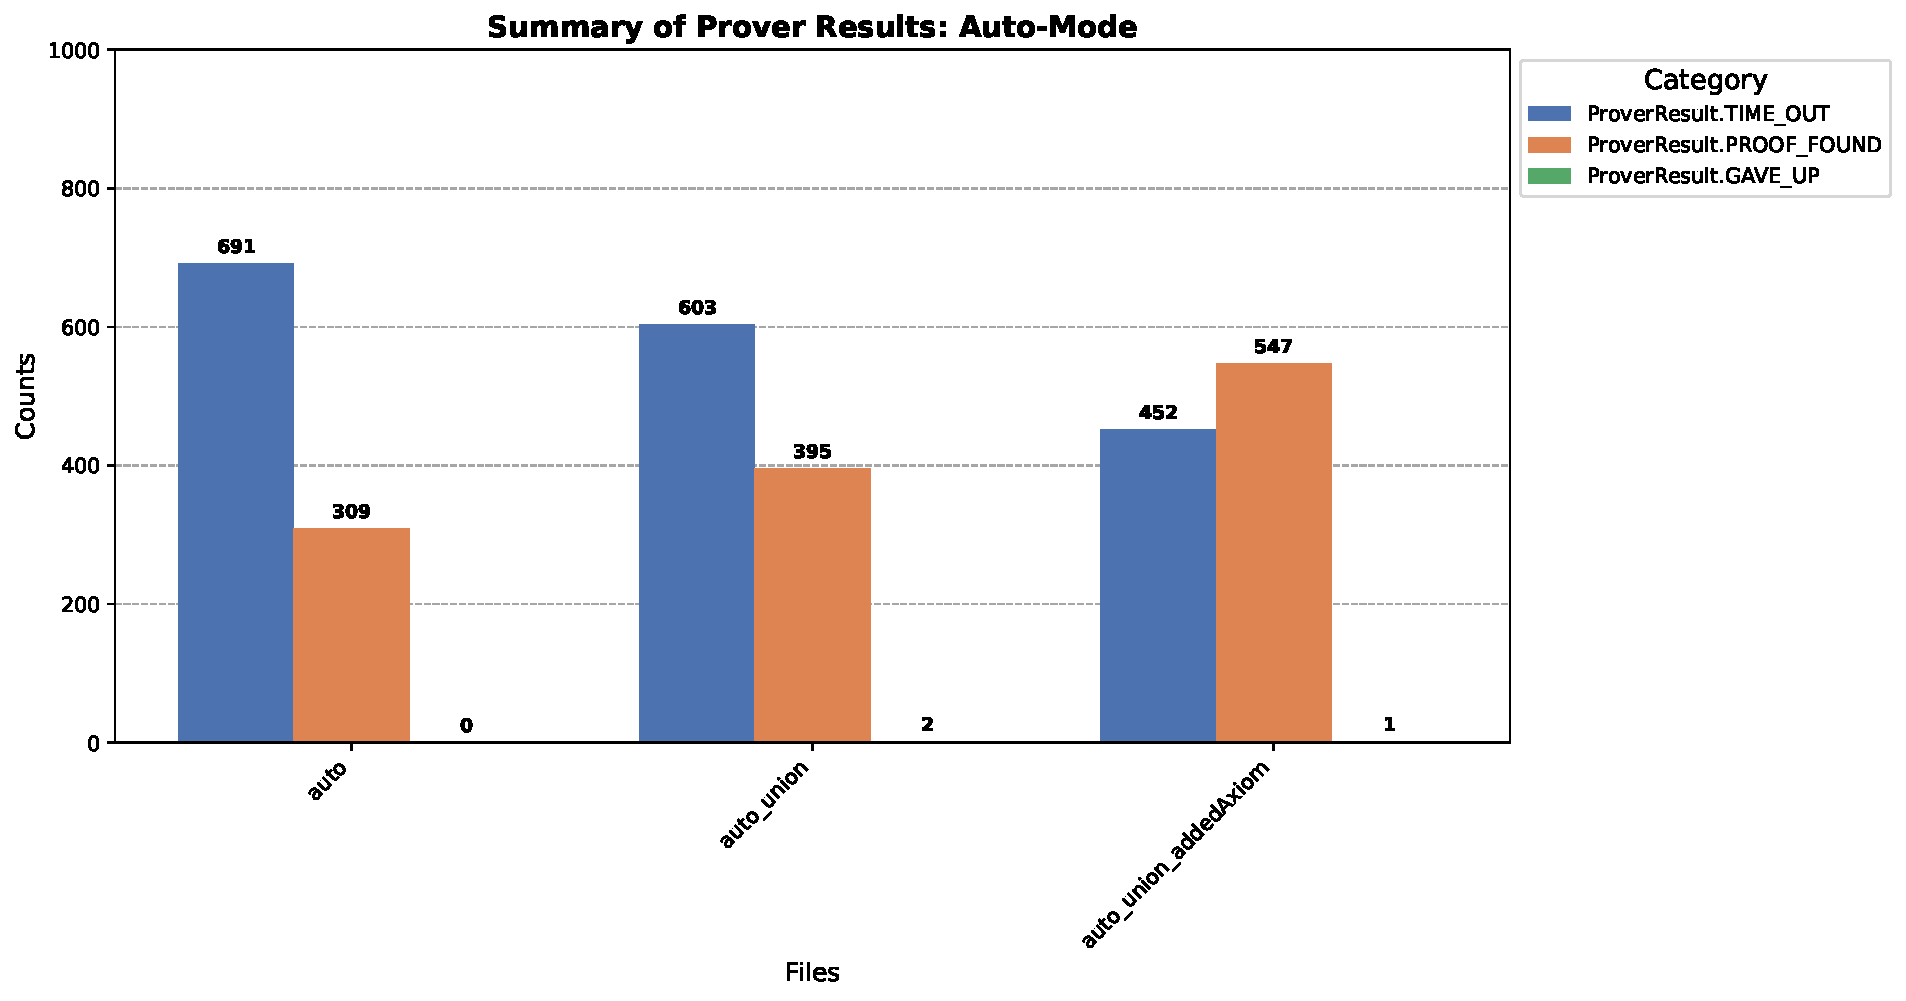
\includegraphics[width=\textwidth]{auto_mode_output.pdf} % Add path to the PDF image
            \caption{Summary of Prover Results: Auto Mode}
            \label{fig:prover_results_auto}
          \end{figure}
          \clearpage
      \end{itemize}
    %
    \section{Different prover}
      \begin{itemize}
        \item Vampire
          \begin{figure}[h!]
            \centering
            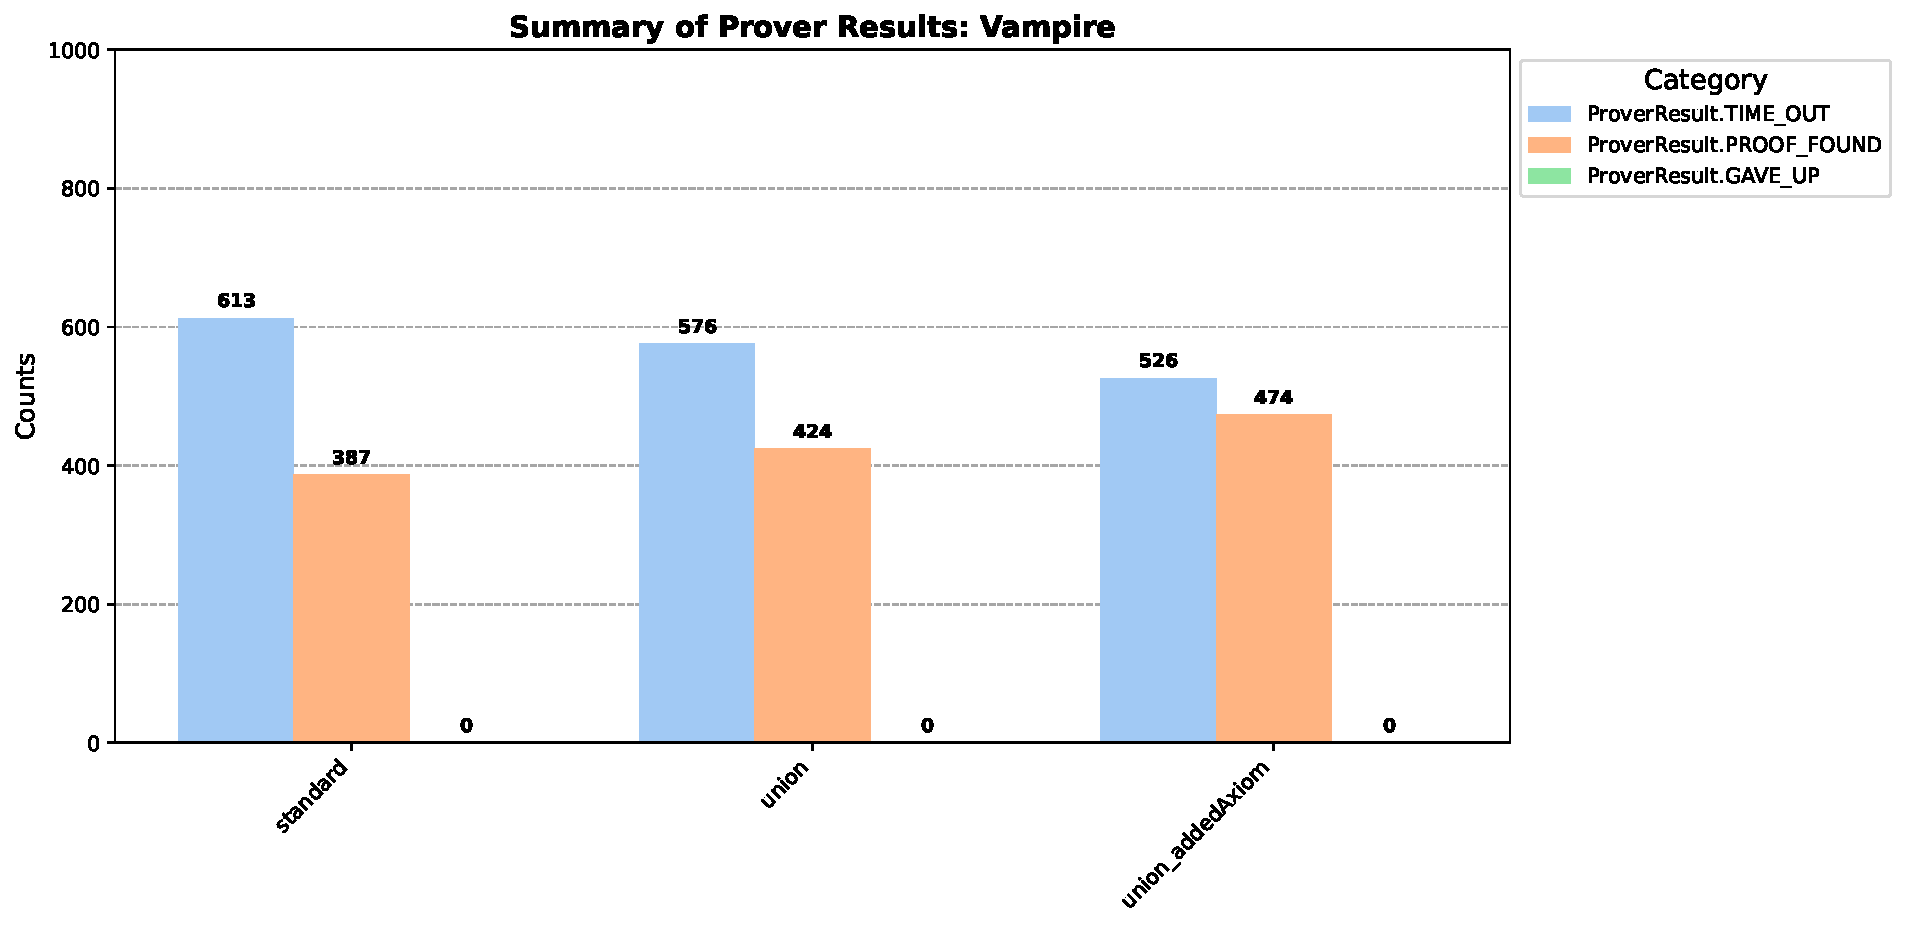
\includegraphics[width=\textwidth]{vampire_mode_output.pdf} % Add path to the PDF image
            \caption{Summary of Prover Results: Vampire Mode}
            \label{fig:prover_results_vampire}
          \end{figure}
          \clearpage
      \end{itemize}
    %
    \section{Time study}
      \begin{itemize}
        \item Proofs found in first named
          \begin{figure}[h!]
            \centering
            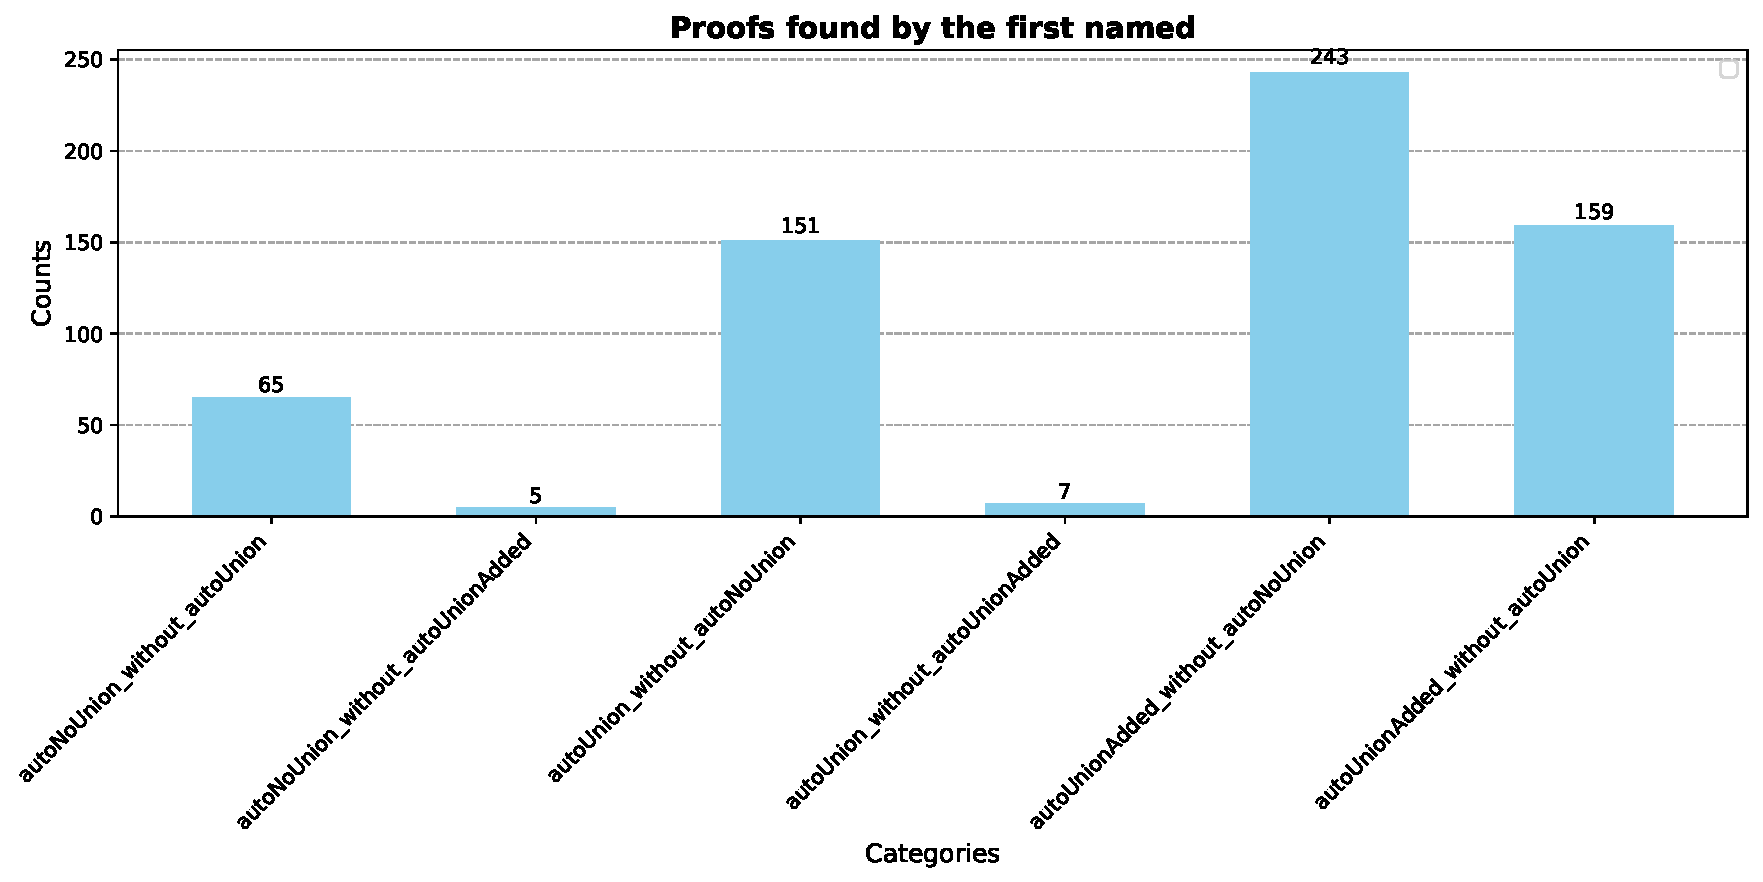
\includegraphics[width=\textwidth]{proof_found_difference.pdf} % Add path to the PDF image
            \caption{Proof found on other modes}
            \label{fig:prover_found_different}
          \end{figure}
        \item Time to find proof
          \begin{figure}[h!]
            \centering
            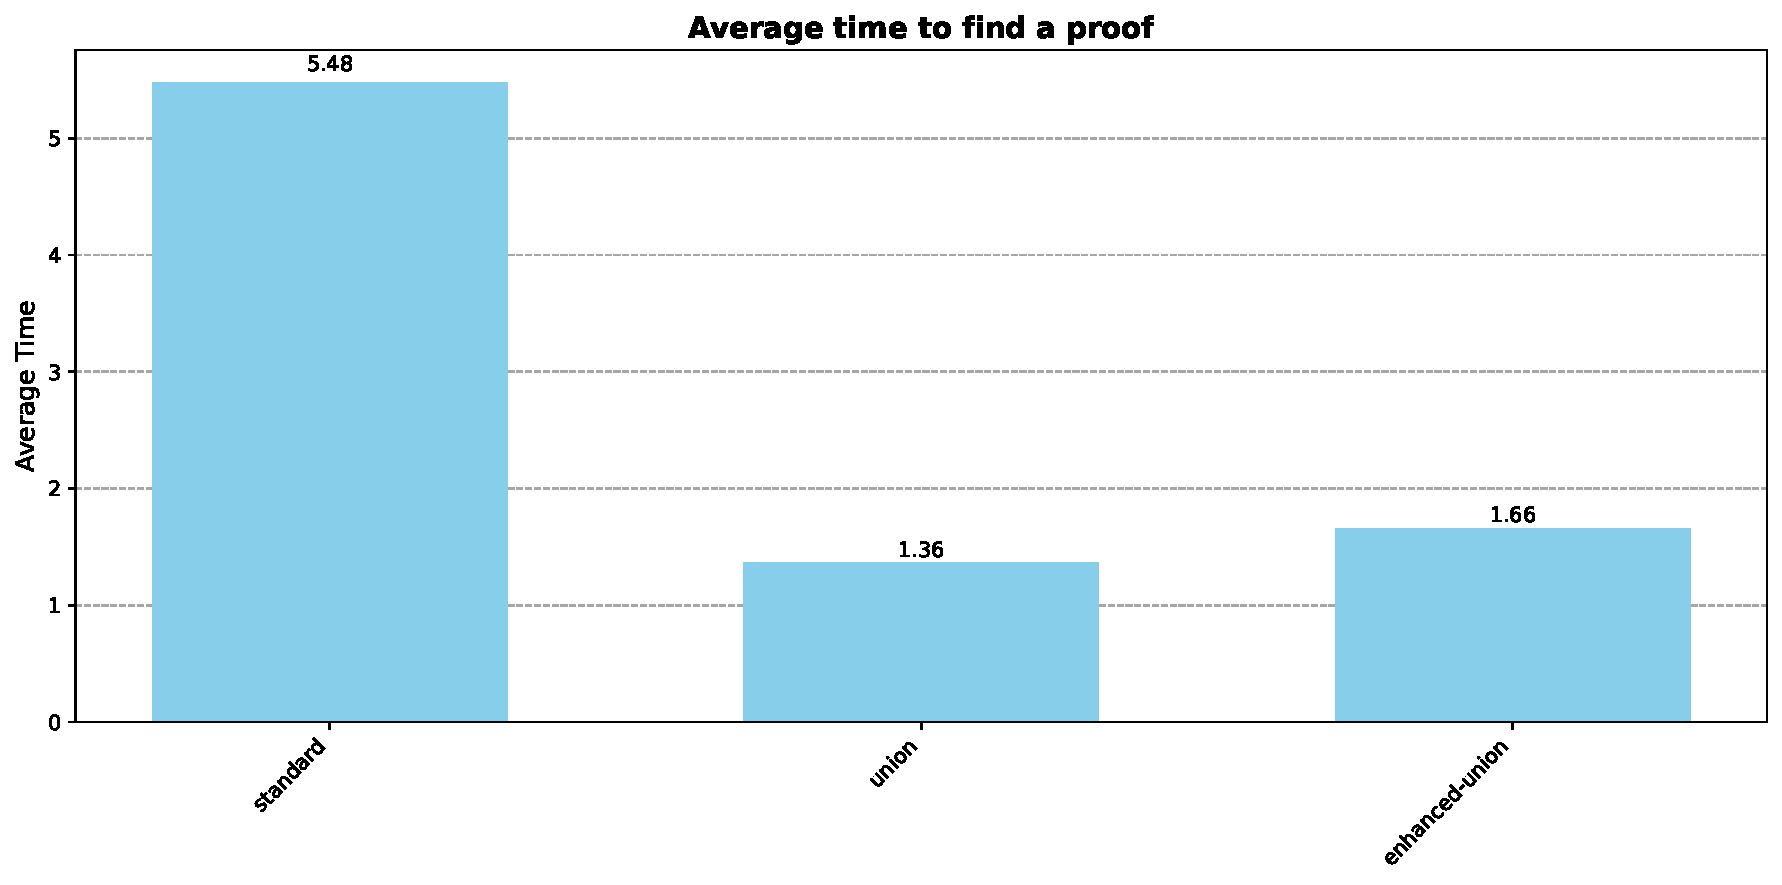
\includegraphics[width=\textwidth]{time_to_find_proof.pdf} % Add path to the PDF image
            \caption{Proofs found time}
            \label{fig:proof_time}
          \end{figure}
        \item Time to find common proof
          \begin{figure}[h!]
            \centering
            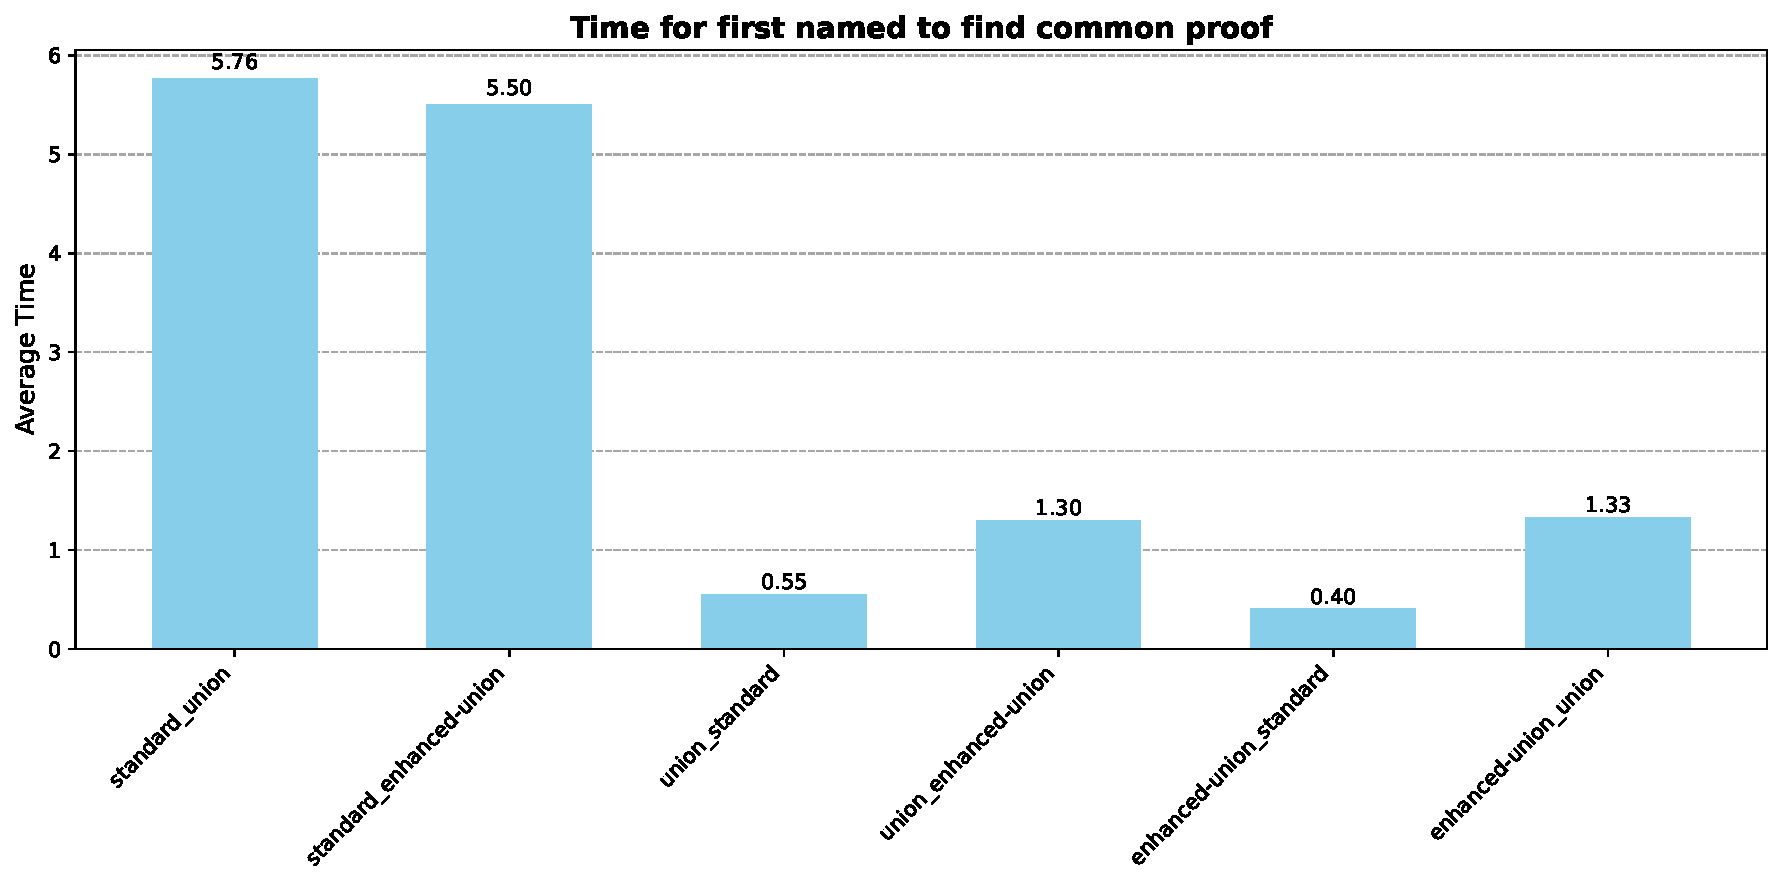
\includegraphics[width=\textwidth]{time_to_find_common_proof.pdf} % Add path to the PDF image
            \caption{Common proofs found time}
            \label{fig:time_common_proof}
          \end{figure}
      \end{itemize}

\chapter{Conclusion}

Conclusion.

\chapter{Further work}

Further work.




% Normally, the bibliography comes next at this point. Do *not* (try
% to) include further indices and tables like an index or
% a list of figures or a list of tables or such things. Nobody
% actually uses them and they just use up space. 
%
% You *can* however include a glossary, if this seems appropriate. It
% goes here as an unnumbered chapter. Most thesis will *not* need a
% glossary: a well-written text (re)explains strange words and
% concepts as necessary. However, there are situations where a
% glossary may be helpful.











|$$|


%%%
% 
% Bibliographies
%
%%%
%
% The uzl-thesis class will load biblatex for the bibliography
% management. This is a powerful package, see its documentation for
% details. The styles will be setup correctly and automatically by
% choosing one of the two style keys as described earlier.
%
% In order for the bibliography to work, run latex in the following
% order (which is the standard order):
% 
% > lualatex thesis-example
% > bibtex thesis-example
% > lualatex thesis-example
% 
% Add BibTeX files using \addbibresource or use the {bibtex entries}
% environment (see below).
%
%%%
%
% Although everyting is normally setup automatically, you can change
% the options passed to biblatex using the key 'biblatex';
% for instance,
%
%   \UzLThesisSetup{biblatex={firstinits=false}}
%
% will switch off shortened first names. Normally, you will not need
% this key in your preamble. 
% 
% Note that the bibtex program is used as the 'backend' of biblatex
% by default (rather than biber, which is the preferred program of
% biblatex). This means that you can (and must) run *bibtex* after you
% have run lualatex on your thesis. If you wish to use biber instead
% of bibtex, say 'biblatex={backend=biber}'. 
% 
%%%
%
% The following environment is optional. It allows you to keep the
% bibtex entries for your thesis right here in the thesis file. What
% happens is that each time this tex file is processed, the contents
% of the following environment gets written to the file
% \jobname-bibtex-entries.bib (this file gets overwritten each
% time). Independently, \addbibresource{\jobname-bibtex-entries.bib}
% is always called if the file \jobname-bibtex-entries.bib
% exists. 
%
% In result, you can edit and keep the bibliography's bibtex entries
% right here. If you change something here, run latex, then bibtex,
% then latex once more.
%
% If you would like to manage the bibtex entries in a separate file,
% remove the below environment, delete the \jobname-bibtex-entries.bib
% file and instead write
%
% \addbibresource{filename-of-your-bibtex-file.bib}
%
% in the preamble.
%
%%%


% !!!!!!!!!!!!!!!!!!!!!!!!!!!!!!!!!!
% !!! Your action is needed here !!!
% !!!!!!!!!!!!!!!!!!!!!!!!!!!!!!!!!!
%
% Replace following example entries with the ones of your thesis.

\begin{bibtex-entries}

@InProceedings{Schon2024,
  author="Jakobs, Oliver
  and Schon, Claudia",
  editor="Hotho, Andreas
  and Rudolph, Sebastian",
  title="Context-Specific Selection of Commonsense Knowledge Using Large Language Models",
  booktitle="KI 2024: Advances in Artificial Intelligence",
  year="2024",
  publisher="Springer Nature Switzerland",
  address="Cham",
  pages="218--231",
  abstract="In the field of automated reasoning, practical applications often face a significant challenge: knowledge bases are typically too large to be fully processed by theorem provers. To still be able to prove that a given goal follows from a large knowledge base, selection techniques are used to determine the parts of the knowledge base that are relevant to the goal. Traditional selection techniques used for this task are usually syntax-based and often overlook a crucial aspect---the meaning of symbol names and axioms. Especially in commonsense reasoning scenarios, the meaning embedded in the symbol names provides invaluable insights. For example, in a proof task using the symbol name cow, it intuitively makes more sense to select formulae using the symbol name calf than formulae using the symbol name weapon. To address this gap, our paper introduces a selection technique that exploits the capabilities of large language models. This technique focuses on contextually related formulae, closely aligning the selected part of the knowledge base with the context of the goal. The approach is implemented and we present a series of experiments that show promising results.",
  isbn="978-3-031-70893-0"
}

@article{Àlvez2014,
  author = {Àlvez, Javier and Lucio, Paqui and Rigau, German},
  year = {2014},
  month = {10},
  pages = {80-116},
  title = {Adimen-SUMO: Reengineering an Ontology for First-Order Reasoning},
  volume = {8},
  journal = {International Journal on Semantic Web and Information Systems},
  doi = {10.4018/jswis.2012100105}
}

@InProceedings{Hoder2011,
  author="Hoder, Kry{\v{s}}tof
  and Voronkov, Andrei",
  editor="Bj{\o}rner, Nikolaj
  and Sofronie-Stokkermans, Viorica",
  title="Sine Qua Non for Large Theory Reasoning",
  booktitle="Automated Deduction -- CADE-23",
  year="2011",
  publisher="Springer Berlin Heidelberg",
  address="Berlin, Heidelberg",
  pages="299--314",
  abstract="One possible way to deal with large theories is to have a good selection method for relevant axioms. This is confirmed by the fact that the largest available first-order knowledge base (the Open CYC) contains over 3 million axioms, while answering queries to it usually requires not more than a few dozen axioms. A method for axiom selection has been proposed by the first author in the Sumo INference Engine (SInE) system. SInE has won the large theory division of CASC in 2008. The method turned out to be so successful that the next two years it was used by the winner as well as by several other competing systems. This paper contains the presentation of the method and describes experiments with it in the theorem prover Vampire.",
  isbn="978-3-642-22438-6"
}

@InProceedings{Roederer2009,
  author="Roederer, Alex
  and Puzis, Yury
  and Sutcliffe, Geoff",
  editor="Schmidt, Renate A.",
  title="Divvy: An ATP Meta-system Based on Axiom Relevance Ordering",
  booktitle="Automated Deduction -- CADE-22",
  year="2009",
  publisher="Springer Berlin Heidelberg",
  address="Berlin, Heidelberg",
  pages="157--162",
  abstract="This paper describes two syntactic relevance orderings on the axioms available for proving a given conjecture, and an ATP meta-system that uses the orderings to select axioms to use in proof attempts. The system has been evaluated, and the results show that it is effective.",
  isbn="978-3-642-02959-2"
}

@InProceedings{Sutcliffe2007,
  author="Sutcliffe, Geoff
  and Puzis, Yury",
  editor="Pfenning, Frank",
  title="SRASS - A Semantic Relevance Axiom Selection System",
  booktitle="Automated Deduction -- CADE-21",
  year="2007",
  publisher="Springer Berlin Heidelberg",
  address="Berlin, Heidelberg",
  pages="295--310",
  abstract="This paper describes the design, implementation, and testing of a system for selecting necessary axioms from a large set also containing superfluous axioms, to obtain a proof of a conjecture. The selection is determined by semantics of the axioms and conjecture, ordered heuristically by a syntactic relevance measure. The system is able to solve many problems that cannot be solved alone by the underlying conventional automated reasoning system.",
  isbn="978-3-540-73595-3"
}

@article{Álvez2017,
  author = {Álvez, Javier and Hermo, Montserrat and Lucio, Paqui and Rigau, German},
  year = {2017},
  month = {05},
  pages = {},
  title = {Automatic White-Box Testing of First-Order Logic Ontologies},
  volume = {29},
  journal = {Journal of Logic and Computation},
  doi = {10.1093/logcom/exz001}
}


\end{bibtex-entries}



% If you need to have an appendix (I advise against it), insert it
% here using, first, \appendix and then \chapter and then,
% possibly, \section. 
%
% \appendix
%
% \chapter{Technical Appendix}
%
% \section{Experimental Parameters} % possibly
%
% Again, I advise against using an appendix.


\end{document}

%  LocalWords:  LaTeX tex moretexcs Lübeck pdf uzl lualatex bibtex th
%  LocalWords:  TechReport Kernighan Lamport's Tantau's Tantau cls kZ
%  LocalWords:  Mustermann emacs oldschool pdflatex texmf utf biber
%  LocalWords:  biblatex Alphabetische Bibliographie Numerische VIIa
%  LocalWords:  varioref german Einleitung Beiträge dieser Arbeit xml
%  LocalWords:  Ergebnisse Verwandte Arbeiten Aufbau nucleotide VIIc
%  LocalWords:  ensembl amino phylogenetic Alexa Siri decrypt versa
%  LocalWords:  cryptographic pre nondeterministic deterministically
%  LocalWords:  Beutelspacher Untersuchungen zum genetischen sep llcc
%  LocalWords:  Beispiel tikz jpg png Alegrya Kasimir Malewitsch PGF
%  LocalWords:  Lamport Institut für Theoretische Informatik zu url
%  LocalWords:  Universität Springer DowneyF Downey Parameterized doi
%  LocalWords:  BibLaTeX Kime Philipp urldate Mittelbach hyperref Lua
%  LocalWords:  Rahtz Oberdiek Heiko Braams Bezos López fontspec Das
%  LocalWords:  Arseneau amsmath ist Tipps und zur Formulierung
%  LocalWords:  mathematischer Gedanken Mathematik Studienanfänger
%  LocalWords:  Albrecht Vieweg Teubner Verlag
